% Options for packages loaded elsewhere
\PassOptionsToPackage{unicode}{hyperref}
\PassOptionsToPackage{hyphens}{url}
\PassOptionsToPackage{dvipsnames,svgnames,x11names}{xcolor}
%
\documentclass[
  letterpaper,
  DIV=11,
  numbers=noendperiod]{scrartcl}

\usepackage{amsmath,amssymb}
\usepackage{iftex}
\ifPDFTeX
  \usepackage[T1]{fontenc}
  \usepackage[utf8]{inputenc}
  \usepackage{textcomp} % provide euro and other symbols
\else % if luatex or xetex
  \usepackage{unicode-math}
  \defaultfontfeatures{Scale=MatchLowercase}
  \defaultfontfeatures[\rmfamily]{Ligatures=TeX,Scale=1}
\fi
\usepackage{lmodern}
\ifPDFTeX\else  
    % xetex/luatex font selection
\fi
% Use upquote if available, for straight quotes in verbatim environments
\IfFileExists{upquote.sty}{\usepackage{upquote}}{}
\IfFileExists{microtype.sty}{% use microtype if available
  \usepackage[]{microtype}
  \UseMicrotypeSet[protrusion]{basicmath} % disable protrusion for tt fonts
}{}
\makeatletter
\@ifundefined{KOMAClassName}{% if non-KOMA class
  \IfFileExists{parskip.sty}{%
    \usepackage{parskip}
  }{% else
    \setlength{\parindent}{0pt}
    \setlength{\parskip}{6pt plus 2pt minus 1pt}}
}{% if KOMA class
  \KOMAoptions{parskip=half}}
\makeatother
\usepackage{xcolor}
\setlength{\emergencystretch}{3em} % prevent overfull lines
\setcounter{secnumdepth}{-\maxdimen} % remove section numbering
% Make \paragraph and \subparagraph free-standing
\ifx\paragraph\undefined\else
  \let\oldparagraph\paragraph
  \renewcommand{\paragraph}[1]{\oldparagraph{#1}\mbox{}}
\fi
\ifx\subparagraph\undefined\else
  \let\oldsubparagraph\subparagraph
  \renewcommand{\subparagraph}[1]{\oldsubparagraph{#1}\mbox{}}
\fi


\providecommand{\tightlist}{%
  \setlength{\itemsep}{0pt}\setlength{\parskip}{0pt}}\usepackage{longtable,booktabs,array}
\usepackage{calc} % for calculating minipage widths
% Correct order of tables after \paragraph or \subparagraph
\usepackage{etoolbox}
\makeatletter
\patchcmd\longtable{\par}{\if@noskipsec\mbox{}\fi\par}{}{}
\makeatother
% Allow footnotes in longtable head/foot
\IfFileExists{footnotehyper.sty}{\usepackage{footnotehyper}}{\usepackage{footnote}}
\makesavenoteenv{longtable}
\usepackage{graphicx}
\makeatletter
\def\maxwidth{\ifdim\Gin@nat@width>\linewidth\linewidth\else\Gin@nat@width\fi}
\def\maxheight{\ifdim\Gin@nat@height>\textheight\textheight\else\Gin@nat@height\fi}
\makeatother
% Scale images if necessary, so that they will not overflow the page
% margins by default, and it is still possible to overwrite the defaults
% using explicit options in \includegraphics[width, height, ...]{}
\setkeys{Gin}{width=\maxwidth,height=\maxheight,keepaspectratio}
% Set default figure placement to htbp
\makeatletter
\def\fps@figure{htbp}
\makeatother
\newlength{\cslhangindent}
\setlength{\cslhangindent}{1.5em}
\newlength{\csllabelwidth}
\setlength{\csllabelwidth}{3em}
\newlength{\cslentryspacingunit} % times entry-spacing
\setlength{\cslentryspacingunit}{\parskip}
\newenvironment{CSLReferences}[2] % #1 hanging-ident, #2 entry spacing
 {% don't indent paragraphs
  \setlength{\parindent}{0pt}
  % turn on hanging indent if param 1 is 1
  \ifodd #1
  \let\oldpar\par
  \def\par{\hangindent=\cslhangindent\oldpar}
  \fi
  % set entry spacing
  \setlength{\parskip}{#2\cslentryspacingunit}
 }%
 {}
\usepackage{calc}
\newcommand{\CSLBlock}[1]{#1\hfill\break}
\newcommand{\CSLLeftMargin}[1]{\parbox[t]{\csllabelwidth}{#1}}
\newcommand{\CSLRightInline}[1]{\parbox[t]{\linewidth - \csllabelwidth}{#1}\break}
\newcommand{\CSLIndent}[1]{\hspace{\cslhangindent}#1}

\KOMAoption{captions}{tableheading}
\makeatletter
\@ifpackageloaded{tcolorbox}{}{\usepackage[skins,breakable]{tcolorbox}}
\@ifpackageloaded{fontawesome5}{}{\usepackage{fontawesome5}}
\definecolor{quarto-callout-color}{HTML}{909090}
\definecolor{quarto-callout-note-color}{HTML}{0758E5}
\definecolor{quarto-callout-important-color}{HTML}{CC1914}
\definecolor{quarto-callout-warning-color}{HTML}{EB9113}
\definecolor{quarto-callout-tip-color}{HTML}{00A047}
\definecolor{quarto-callout-caution-color}{HTML}{FC5300}
\definecolor{quarto-callout-color-frame}{HTML}{acacac}
\definecolor{quarto-callout-note-color-frame}{HTML}{4582ec}
\definecolor{quarto-callout-important-color-frame}{HTML}{d9534f}
\definecolor{quarto-callout-warning-color-frame}{HTML}{f0ad4e}
\definecolor{quarto-callout-tip-color-frame}{HTML}{02b875}
\definecolor{quarto-callout-caution-color-frame}{HTML}{fd7e14}
\makeatother
\makeatletter
\makeatother
\makeatletter
\makeatother
\makeatletter
\@ifpackageloaded{caption}{}{\usepackage{caption}}
\AtBeginDocument{%
\ifdefined\contentsname
  \renewcommand*\contentsname{Table of contents}
\else
  \newcommand\contentsname{Table of contents}
\fi
\ifdefined\listfigurename
  \renewcommand*\listfigurename{List of Figures}
\else
  \newcommand\listfigurename{List of Figures}
\fi
\ifdefined\listtablename
  \renewcommand*\listtablename{List of Tables}
\else
  \newcommand\listtablename{List of Tables}
\fi
\ifdefined\figurename
  \renewcommand*\figurename{Figure}
\else
  \newcommand\figurename{Figure}
\fi
\ifdefined\tablename
  \renewcommand*\tablename{Table}
\else
  \newcommand\tablename{Table}
\fi
}
\@ifpackageloaded{float}{}{\usepackage{float}}
\floatstyle{ruled}
\@ifundefined{c@chapter}{\newfloat{codelisting}{h}{lop}}{\newfloat{codelisting}{h}{lop}[chapter]}
\floatname{codelisting}{Listing}
\newcommand*\listoflistings{\listof{codelisting}{List of Listings}}
\makeatother
\makeatletter
\@ifpackageloaded{caption}{}{\usepackage{caption}}
\@ifpackageloaded{subcaption}{}{\usepackage{subcaption}}
\makeatother
\makeatletter
\makeatother
\ifLuaTeX
  \usepackage{selnolig}  % disable illegal ligatures
\fi
\IfFileExists{bookmark.sty}{\usepackage{bookmark}}{\usepackage{hyperref}}
\IfFileExists{xurl.sty}{\usepackage{xurl}}{} % add URL line breaks if available
\urlstyle{same} % disable monospaced font for URLs
\hypersetup{
  pdftitle={Graph embedding and transfer learning can help predict potential species interaction networks despite data limitations},
  colorlinks=true,
  linkcolor={blue},
  filecolor={Maroon},
  citecolor={Blue},
  urlcolor={Blue},
  pdfcreator={LaTeX via pandoc}}

\title{Graph embedding and transfer learning can help predict potential
species interaction networks despite data limitations}
\author{Tanya Strydom \and Salomé Bouskila \and Francis
Banville \and Ceres Barros \and Dominique Caron \and Maxwell J.
Farrell \and Marie-Josée Fortin \and Benjamin Mercier \and Laura J.
Pollock \and Rogini Runghen \and Giulio V. Dalla Riva \and Timothée
Poisot}
\date{}

\begin{document}
\maketitle
\begin{abstract}
\begin{itemize}
\tightlist
\item
  Metawebs (networks of potential interactions within a species pool)
  are a powerful abstraction to understand how large-scale species
  interaction networks are structured.
\item
  Because metawebs are typically expressed at large spatial and
  taxonomic scales, assembling them is a tedious and costly process;
  predictive methods can help circumvent the limitations in data
  deficiencies, by providing a first approximation of metawebs.''
\item
  One way to improve our ability to predict metawebs is to maximize
  available information by using graph embeddings, as opposed to an
  exhaustive list of species interactions. Graph embedding is an
  emerging field in machine learning that holds great potential for
  ecological problems.
\item
  Here, we outline how the challenges associated with inferring metawebs
  line-up with the advantages of graph embeddings; followed by a
  discussion as to how the choice of the species pool has consequences
  on the reconstructed network, specifically as to the role of
  human-made (or arbitrarily assigned) boundaries and how these may
  influence ecological hypotheses.
\end{itemize}
\end{abstract}
The ability to infer potential biotic interactions could serve as a
significant breakthrough in our ability to conceptualize networks over
large spatial scales (Hortal et al. 2015). Reliable inferences would not
only boost our understanding of the structure of species interaction
networks, but also increase the amount of information that can be used
for biodiversity management. In a recent overview of the field of
ecological network prediction, Strydom et al. (2021) identified two
challenges of interest to the prediction of interactions at large
scales. First, there is a relative scarcity of relevant data in most
places globally -- which, due to the limitations in most predictive
methods, restricts the ability to infer interactions to locations where
it is least required (\emph{i.e.} regions where we already have
interaction data) leaving us unable to make inference in data scarce
regions (where we most need it); second, accurate predictors are
important for accurate predictions, and the lack of methods that can
leverage a small amount of \emph{accurate} data is a serious impediment
to our predictive ability. In this contribution, we (i) highlight the
power of viewing (and constructing) metawebs as \emph{probabilistic}
objects in the context of low-probability interactions, (ii) discuss how
a family of machine learning tools (graph embeddings and transfer
learning) can be used to overcome data limitations to metaweb inference,
and (iii) highlight how the use of metawebs introduces important
questions for the field of network ecology.

In most places, our most reliable biodiversity knowledge is that of a
species pool where a set of potentially interacting species in a given
area could occur: through the analysis of databases like the Global
Biodiversity Information Facility (GBIF) or the International Union for
the Conservation of Nature (IUCN), it is possible to construct a list of
species for a region of interest. Following the definition of Dunne
(2006), a metaweb is the ecological network analogue to the species
pool; specifically, it inventories all \emph{potential} interactions
between species for a spatially delimited area (and so captures the
\(\gamma\) diversity of interactions as per Poisot et al. (2012)).
However, inferring the potential interactions between these species
still remains a challenge. And yet, the metaweb holds valuable
ecological information: it represents the joint effect of functional,
phylogenetic, and macroecological processes (Morales-Castilla et al.
2015; Carlson et al. 2022; Morales-Castilla et al. 2021). Specifically,
it represents the ``upper bounds'' on what the composition of the local
networks, given a local species pool, can be (see \emph{e.g.} McLeod et
al. 2021); this information can help evaluate the ability of ecological
assemblages to withstand the effects of, for example, climate change
(Fricke et al. 2022). These local networks may be reconstructed given an
appropriate knowledge of local species composition and provide
information on the structure of networks at finer spatial scales. This
has been done for example for tree-galler-parasitoid systems (Gravel et
al. 2018), fish trophic interactions (Albouy et al. 2019), terrestrial
tetrapod trophic interactions (J. Braga et al. 2019; O'Connor et al.
2020), and crop-pest networks (Grünig et al. 2020).

The metaweb itself is not a prediction of local networks at specific
locations within the spatial area it covers: it will have a different
structure, notably by having a larger connectance (see \emph{e.g.} Wood
et al. 2015) and complexity (see \emph{e.g.} Galiana et al. 2022), than
any of these local networks. Local networks (which capture the
\(\alpha\) diversity of interactions) are a subset of the metaweb's
species and its realized interactions, and have been called ``metaweb
realizations'' (Poisot, Stouffer, and Gravel 2015). Differences between
local networks and their metawebs are due to chance, species abundance
and co-occurrence, local environmental conditions, and local
distribution of functional traits, among others. Specifically, although
co-occurrence can be driven by interactions (Cazelles et al. 2016),
co-occurrence alone is not a predictor of interactions (Blanchet,
Cazelles, and Gravel 2020; Thurman et al. 2019), and therefore the lack
of co-occurrence cannot be used to infer the lack of a feasible
interaction. Yet, recent results by Saravia et al. (2021) strongly
suggested that local (metaweb) realizations only respond weakly to local
conditions: instead, they reflect constraints inherited by the structure
of their metaweb. This sets up the core goal of predictive network
ecology as the prediction of metaweb structure, as it is required to
accurately produce downscaled, local predictions.

\hypertarget{a-metaweb-is-an-inherently-probabilistic-object}{%
\section{A metaweb is an inherently probabilistic
object}\label{a-metaweb-is-an-inherently-probabilistic-object}}

Treating interactions as probabilistic (as opposed to binary) events is
a more nuanced and realistic way to represent them. Dallas, Park, and
Drake (2017) suggested that most interactions (links) in ecological
networks are cryptic, \emph{i.e.} uncommon or hard to observe. This
argument echoes Jordano (2016): sampling ecological interactions is
difficult because it requires first the joint observation of two
species, and then the observation of their interaction. In addition, it
is generally expected that weak or rare interactions will be more
prevalent in networks than common or strong interactions (Csermely
2004); this is notably the case in food chains, wherein many weaker
interactions are key to the stability of a system (Neutel, Heesterbeek,
and de Ruiter 2002). In the light of these observations, we expect to
see an over-representation of low-probability (hereafter rare)
interactions under a model that accurately predicts interaction
probabilities.

Yet, the original metaweb definition, and indeed most past uses of
metawebs, was based on the presence/absence of interactions. Moving
towards \emph{probabilistic} metawebs, by representing interactions as
Bernoulli events (see \emph{e.g.} Poisot et al. 2016), offers the
opportunity to weigh these rare interactions appropriately. The inherent
plasticity of interactions is important to capture: there have been
documented instances of food webs undergoing rapid collapse/recovery
cycles over short periods of time (\emph{e.g.} Pedersen et al. 2017).
Furthermore, because the structure of the metaweb cannot be known in
advance, it is important to rely on predictive tools that do not assume
a specific network topology for link prediction (Gaucher, Klopp, and
Robin 2021), but are able to work on generalizations of the network that
capture statistical processes giving it its structure. These
considerations emphasize why metaweb predictions should focus on
quantitative (preferentially probabilistic) predictions, and this should
constrain the suite of models that are appropriate for prediction.
Binary classifiers based on probabilities have an extremely robust
methodology to validate them, and this applies naturally to the
prediction of interactions (Poisot 2023).

It is important to recall that a metaweb is intended as a catalogue of
all potential (feasible) interactions, which is then filtered for a
given application (Morales-Castilla et al. 2015). It is therefore
important to separate the interactions that happen ``almost surely''
(repeated observational data), ``almost never'' (repeated lack of
evidence \emph{or} evidence that the link is forbidden through
\emph{e.g.} trait mis-match), and interactions with a probability that
lays somewhere in between (Catchen et al. 2023). Although metawebs can
(and in practice likely do) include false positives, these are
statistically negligible compared to the false negatives. Furthermore,
Strydom et al. (2022) shows that t-SVD embedding is extremely robust to
(and able to detect) the presence of false positives. In a sense,
because most ecological interactions are elusive, we should consider the
direct consequences this has on sampling: once the common interactions
are documented, the effort required in documenting each rare interaction
will increase exponentially (Jordano 2016). Recent proposals in other
fields relying on machine learning approaches emphasize the idea that
algorithms meant to predict, through the assumption that they
approximate the process generating the data, can also act as data
generators (Hoffmann et al. 2019). High quality observational data can
be used to infer core rules underpinning network structure, and be
supplemented with synthetic data coming from predictive models trained
on them, thereby increasing the volume of information available for
analysis. Indeed, Strydom et al. (2021) suggested that knowing the
metaweb may render the prediction of local networks easier, because it
fixes an ``upper bound'' on which interactions can exist. In this
context, a probabilistic metaweb represents an aggregation of
informative priors on the biological feasibility of interactions, which
is usually hard to obtain yet has possibly the most potential to boost
our predictive ability of local networks (Bartomeus 2013; Bartomeus et
al. 2016). This would represent a departure from simple rules expressed
at the network scale (\emph{e.g.} Williams and Martinez 2000) to a view
of network prediction based on learning the rules that underpin
interactions \emph{and} their variability (Anubhav Gupta, Furrer, and
Petchey 2022).

\begin{figure}

{\centering 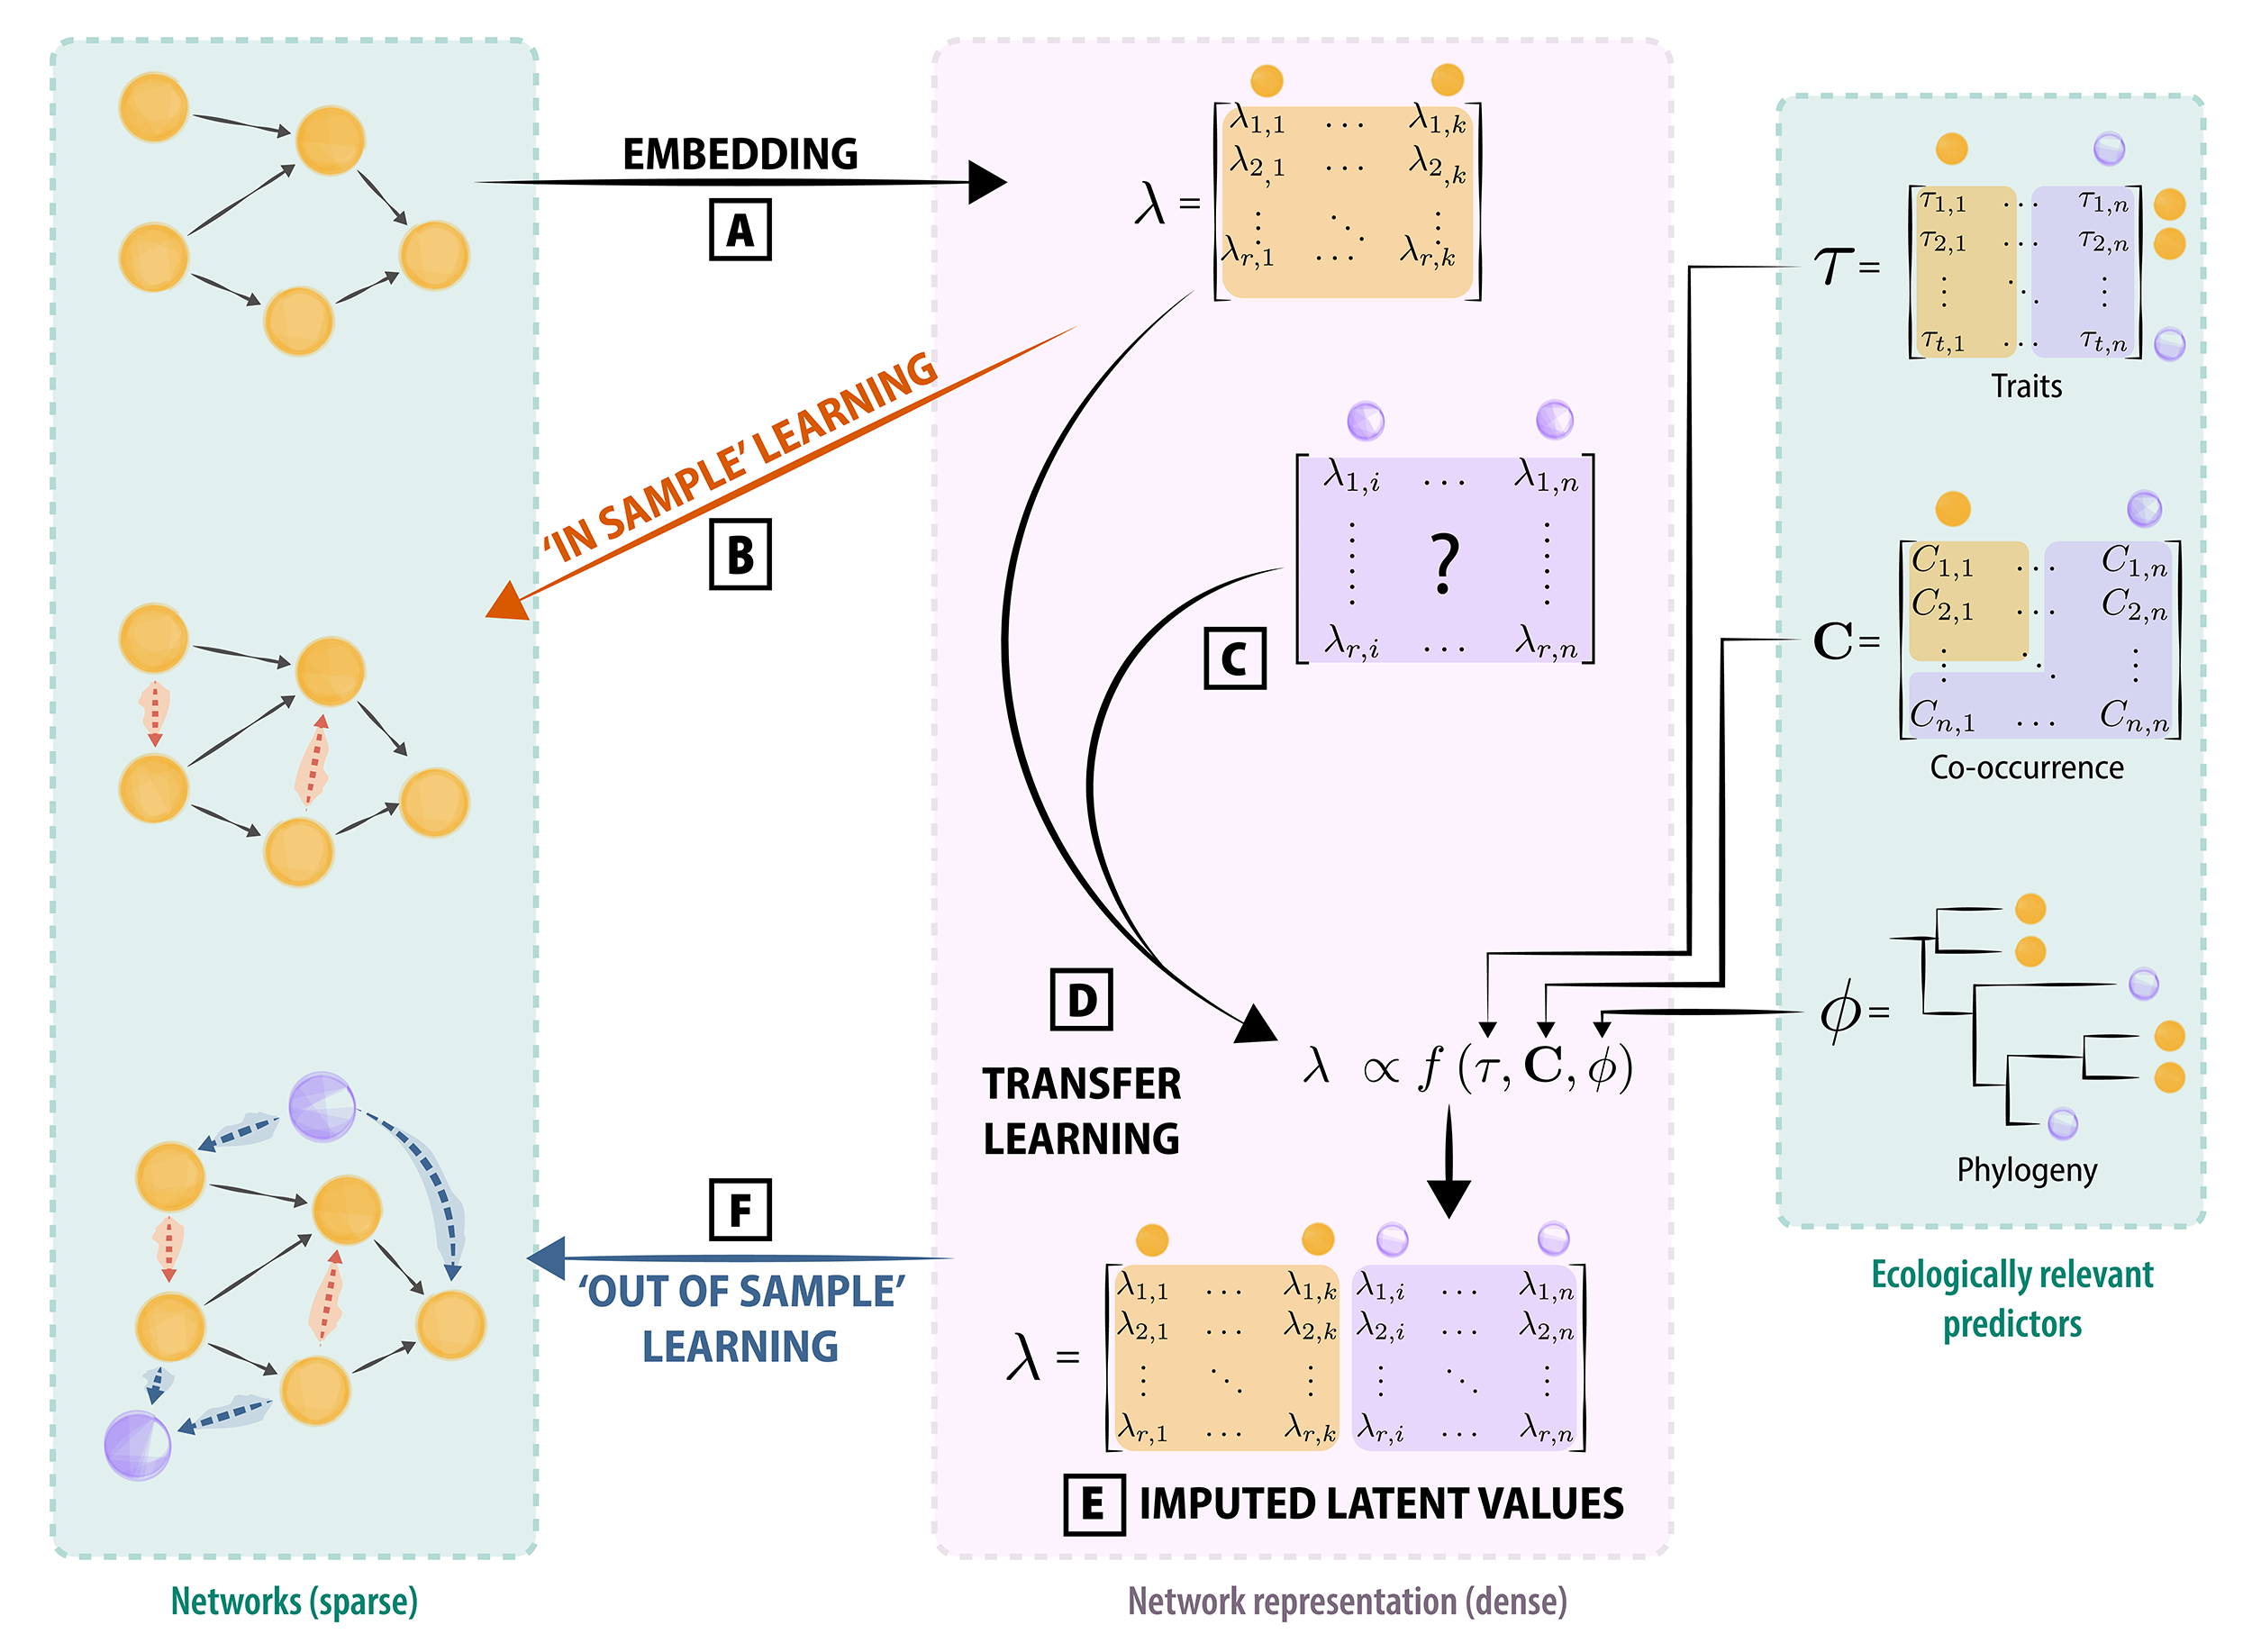
\includegraphics{figures/conceptual_2.png}

}

\caption{\label{fig-embedding}The embedding process (\textbf{A}) can
help to identify links (interactions) that may have been missed within
the original community (represented by the orange dashed arrows,
\textbf{B}). Transfer learning (\textbf{D}) allows for the prediction of
links (interactions) even when novel species (\textbf{C}) are included
alongside the original community. This is achieved with other
ecologically relevant predictors (\emph{e.g.} traits) in conjunction
with the known interactions to infer latent values (\textbf{E}).
Ultimately this allows us to predict links (interactions) for species
external from the original sample (blue dashed arrows) as well as
missing within sample links (\textbf{F}). Within this context the
predicted (and original) networks as well as the ecological predictors
used (green boxes) are products that can be quantified through
measurements in the field, whereas the embedded as well as imputed
matrices (purple box) are representative of a decomposition of the
interaction matrices onto the embedding space}

\end{figure}

\hypertarget{graph-embedding-offers-promises-for-the-inference-of-potential-interactions}{%
\section{Graph embedding offers promises for the inference of potential
interactions}\label{graph-embedding-offers-promises-for-the-inference-of-potential-interactions}}

Graph (or network) embedding (Figure~\ref{fig-embedding}) is a family of
machine learning techniques, whose main task is to learn a mapping
function from a discrete graph to a continuous domain (Arsov and Mirceva
2019; Chami et al. 2022). Their main goal is to learn a low dimensional
vector representation of the graph (embeddings), such that its key
properties (\emph{e.g.} local or global structures) are retained in the
embedding space (Yan et al. 2005). The embedding space may, but will not
necessarily, have lower dimensionality than the graph. Ecological
networks are promising candidates for the routine application of
embeddings, as they tend to possess a shared structural backbone (see
\emph{e.g.} Bramon Mora et al. 2018), which hints at structural
invariants in empirical data. Assuming that these structural invariants
are common enough, they would dominate the structure of networks, and
therefore be adequately captured by the first (lower) dimensions of an
embedding, without the need to measure derived aspects of their
structure (\emph{e.g.} motifs, paths, modularity, \ldots).

\hypertarget{graph-embedding-produces-latent-variables-but-not-traits}{%
\subsection{Graph embedding produces latent variables (but not
traits)}\label{graph-embedding-produces-latent-variables-but-not-traits}}

Before moving further, it is important to clarify the epistemic status
of node values derived from embeddings: specifically, they are
\emph{not} functional traits, and therefore should not be interpreted in
terms of effects or responses. As per the framework of Malaterre et al.
(2019), these values neither derive from, nor result in, changes in
organismal performance, and should therefore not be used to quantify
\emph{e.g.} functional diversity. This holds true even when there are
correlations between latent values and functional traits: although these
enable an ecological discussion of how traits condition the structure of
the network, the existence of a statistical relationship does not
elevate the latent values to the status of functional traits.

Rather than directly predicting biological rules (see \emph{e.g.}
Pichler et al. 2020 for an overview), which may be confounded by the
sparse nature of graph data, learning embeddings works in the
low-dimensional space that maximizes information about the network
structure. This approach is further justified by the observation, for
example, that the macro-evolutionary history of a network is adequately
represented by some graph embeddings {[}Random dot product graphs
(RDPG); see Dalla Riva and Stouffer (2016){]}. In a recent publication,
Strydom et al. (2022) have used an embedding (based on RDPG) to project
a metaweb of trophic interactions between European mammals, and
transferred this information to mammals of Canada, using the
phylogenetic distance between related clades to infer the values in the
latent subspace into which the European metaweb was projected. By
performing the RDPG step on re-constructed values, this approach yields
a probabilistic trophic metaweb for mammals of Canada based on knowledge
of European species, despite a limited (\(\approx\) 5\%) taxonomic
overlap, and illustrates how the values derived from an embedding can be
used for prediction without being ``traits'' of the species they
represent.

\hypertarget{ecological-networks-are-good-candidates-for-embedding}{%
\subsection{Ecological networks are good candidates for
embedding}\label{ecological-networks-are-good-candidates-for-embedding}}

Ecological networks are inherently low-dimensional objects, and can be
adequately represented with less than ten dimensions (M. P. Braga et al.
2021; Eklöf et al. 2013; J. Braga et al. 2019). Simulation results by
Botella et al. (2022) suggested that there is no dominant method to
identify architectural similarities between networks: multiple
approaches need to be tested and compared to the network descriptor of
interest on a problem-specific basis. This matches previous results on
graph embedding, wherein different embedding algorithms yield different
network embeddings (Goyal and Ferrara 2018), calling for a careful
selection of the problem-specific approach to use. Additionally,
Ghasemian et al. (2020) suggest that in some cases, nodes embeddings can
be outperformed by other methods, re-inforcing the need to thoroughly
select the appropriate data analysis technique. In
Table~\ref{tbl-methods}, we present a selection of common graph and node
embedding methods, alongside examples of their use to predict
interactions or statistical associations between species. These methods
rely largely on linear algebra or pseudo-random walks on graphs. All
forms of embeddings presented in Table~\ref{tbl-methods} share the
common property of summarizing their objects into (sets of) dense
feature vectors, that capture the overall network structure, pairwise
information on nodes, and emergent aspects of the network, in a
compressed way (\emph{i.e.} with some information loss, as we later
discuss in the illustration). Node embeddings tend to focus on
maintaining pairwise relationships (\emph{i.e.} species interactions),
while graph embeddings focus on maintaining the network structure
(\emph{i.e.} emergent properties). Nevertheless, some graph embedding
techniques (like RDPG, see \emph{e.g.} Wu, Palmer, and Deford 2021) will
provide high-quality node-level embeddings while also preserving network
structure.

\begin{tcolorbox}[enhanced jigsaw, coltitle=black, title=\textcolor{quarto-callout-note-color}{\faInfo}\hspace{0.5em}{Box 1 - Graph Neural Networks}, bottomtitle=1mm, colback=white, breakable, colbacktitle=quarto-callout-note-color!10!white, opacityback=0, left=2mm, arc=.35mm, colframe=quarto-callout-note-color-frame, toptitle=1mm, leftrule=.75mm, rightrule=.15mm, titlerule=0mm, bottomrule=.15mm, toprule=.15mm, opacitybacktitle=0.6]

One prominent family of approaches we do not discuss in the present
manuscript is Graph Neural Networks {[}GNN; Zhou et al. (2020){]}. GNN
are, in a sense, a method to embed a graph into a dense subspace, but
belong to the family of deep learning methods, which has its own set of
practices (see \emph{e.g.} Goodfellow, Bengio, and Courville 2016). An
important issue with methods based on deep learning is that, because
their parameter space is immense, the sample size of the data fed into
them must be similarly large (typically thousands of instances). This is
a requirement for the model to converge correctly during training, but
this assumption is unlikely to be met given the size of datasets
currently available for metawebs (or single time/location species
interaction networks). This data volume requirement is mostly absent
from the techniques we list below. Furthermore, GNN still have some
challenges related to their shallow structure, and concerns related to
scalability (see Atika Gupta, Matta, and Pant 2021 for a review), which
are mostly absent from the methods listed in Table~\ref{tbl-methods}.
Assuming that the uptake of next-generation biomonitoring techniques
does indeed deliver larger datasets on species interactions (Bohan et
al. 2017), there is nevertheless the potential for GNN to become an
applicable embedding/predictive technique in the coming years.

\end{tcolorbox}

Graph embeddings \emph{can} serve as a dimensionality reduction method.
For example, RDPG (Strydom et al. 2022) and t-SVD {[}truncated Singular
Value Decomposition; Poisot et al. (2021){]} typically embed networks
using fewer dimensions than the original network {[}the original network
has as many dimensions as species, and as many informative dimensions as
trophically unique species; Strydom, Dalla Riva, and Poisot (2021){]}.
However, this is not necessarily the case -- indeed, one may perform a
PCA (a special case of SVD) to project the raw data into a subspace that
improves the efficacy of t-SNE {[}t-distributed stochastic neighbor
embedding; Maaten (2009){]}. There are many dimensionality reductions
(Anowar, Sadaoui, and Selim 2021) that can be applied to an embedded
network should the need for dimensionality reduction (for example for
data visualization) arise. In brief, many graph embeddings \emph{can}
serve as dimensionality reduction steps, but not all do, neither do all
dimensionality reduction methods provide adequate graph embedding
capacities. In the next section (and Figure~\ref{fig-embedding}), we
show how the amount of dimensionality reduction can affect the quality
of the embedding.

\hypertarget{tbl-methods}{}
\begin{longtable}[]{@{}
  >{\raggedright\arraybackslash}p{(\columnwidth - 8\tabcolsep) * \real{0.2000}}
  >{\raggedright\arraybackslash}p{(\columnwidth - 8\tabcolsep) * \real{0.2000}}
  >{\raggedright\arraybackslash}p{(\columnwidth - 8\tabcolsep) * \real{0.2000}}
  >{\raggedright\arraybackslash}p{(\columnwidth - 8\tabcolsep) * \real{0.2000}}
  >{\raggedright\arraybackslash}p{(\columnwidth - 8\tabcolsep) * \real{0.2000}}@{}}
\caption{\label{tbl-methods}Overview of some common graph embedding
approaches, by type of embedded objects, alongside examples of their use
in the prediction of species interactions. These methods have not yet
been routinely used to predict species interactions; most examples that
we identified were either statistical associations, or analogues to
joint species distribution models. \(^a\): application is concerned with
\emph{statistical} interactions, which are not necessarilly direct
biotic interactions; \(^b\):application is concerned with joint-SDM-like
approach, which is also very close to statistical associations as
opposed to direct biotic interactions. Given the need to evaluate
different methods on a problem-specific basis, the fact that many
methods have not been used on network problems is an opportunity for
benchmarking and method development. Note that the row for PCA also
applies to kernel/probabilistic PCA, which are variations on the more
general method of SVD. Note further that t-SNE has been included because
it is frequently used to embed graphs, including of species
associations/interactions, despite not being strictly speaking, a graph
embedding technique (see \emph{e.g.} Chami et al. 2022).}\tabularnewline
\toprule\noalign{}
\begin{minipage}[b]{\linewidth}\raggedright
Method
\end{minipage} & \begin{minipage}[b]{\linewidth}\raggedright
Object
\end{minipage} & \begin{minipage}[b]{\linewidth}\raggedright
Technique
\end{minipage} & \begin{minipage}[b]{\linewidth}\raggedright
Reference
\end{minipage} & \begin{minipage}[b]{\linewidth}\raggedright
Application
\end{minipage} \\
\midrule\noalign{}
\endfirsthead
\toprule\noalign{}
\begin{minipage}[b]{\linewidth}\raggedright
Method
\end{minipage} & \begin{minipage}[b]{\linewidth}\raggedright
Object
\end{minipage} & \begin{minipage}[b]{\linewidth}\raggedright
Technique
\end{minipage} & \begin{minipage}[b]{\linewidth}\raggedright
Reference
\end{minipage} & \begin{minipage}[b]{\linewidth}\raggedright
Application
\end{minipage} \\
\midrule\noalign{}
\endhead
\bottomrule\noalign{}
\endlastfoot
t-SNE & nodes & statistical divergence & Hinton and Roweis (2002) &
(Cieslak et al. 2020, species-environment responses \(^a\)) (Gibb et al.
2021, host-virus network representation) \\
LINE & nodes & stochastic gradient descent & Tang et al. (2015) & \\
SDNE & nodes & gradient descent & D. Wang, Cui, and Zhu (2016) & \\
node2vec & nodes & stochastic gradient descent & Grover and Leskovec
(2016) & \\
HARP & nodes & meta-strategy & H. Chen et al. (2017) & \\
DMSE & joint nodes & deep neural network & D. Chen et al. (2017) & (D.
Chen et al. 2017, species-environment interactions \(^b\)) \\
graph2vec & sub-graph & skipgram network & Narayanan et al. (2017) & \\
RDPG & graph & SVD & Young and Scheinerman (2007) & (Dalla Riva and
Stouffer 2016, trophic interactions) (Poisot et al. 2021, host-virus
network prediction) \\
GLEE & graph & Laplacian eigenmap & Torres, Chan, and Eliassi-Rad (2020)
& \\
DeepWalk & graph & stochastic gradient descent & Perozzi, Al-Rfou, and
Skiena (2014) & (Wardeh, Baylis, and Blagrove 2021, host-virus
interactions) \\
GraphKKE & graph & stochastic differential equation & Melnyk et al.
(2020) & (Melnyk et al. 2020, microbiome species associations \(^a\)) \\
FastEmbed & graph & eigen decomposition & Ramasamy and Madhow (2015)
& \\
PCA & graph & eigen decomposition & Surendran (2013) & (Strydom et al.
2021, host-parasite interactions) \\
Joint methods & multiple graphs & multiple strategies & S. Wang et al.
(2021) & \\
\end{longtable}

The popularity of graph embedding techniques in machine learning is more
than the search for structural invariants: graphs are discrete objects,
and machine learning techniques tend to handle continuous data better.
Bringing a sparse graph into a continuous, dense vector space (Xu 2021)
opens up a broader variety of predictive algorithms, notably of the sort
that are able to predict events as probabilities (Murphy 2022).
Furthermore, the projection of the graph itself is a representation that
can be learned; Runghen, Stouffer, and Dalla Riva (2021), for example,
used a neural network to learn the embedding of a network in which not
all interactions were known, based on the nodes' metadata. This example
has many parallels in ecology (see Figure~\ref{fig-embedding}
\textbf{C}), in which node metadata can be represented by phylogeny,
abundance, or functional traits. Using phylogeny as a source of
information assumes (or strives to capture) the action of evolutionary
processes on network structure, which at least for networks have been
well documented (M. P. Braga et al. 2021; Dalla Riva and Stouffer 2016;
Eklöf and Stouffer 2016; D. B. Stouffer et al. 2007; D. B. Stouffer et
al. 2012); similarly, the use of functional traits assumes that
interactions can be inferred from the knowledge of trait-matching rules,
which is similarly well supported in the empirical literature (Bartomeus
2013; Bartomeus et al. 2016; Goebel et al. 2023; Gravel et al. 2013).
Relating this information to an embedding rather than a list of network
measures would allow to capture their effect on the more fundamental
aspects of network structure; conversely, the absence of a phylogenetic
or functional signal may suggest that evolutionary/trait processes are
not strong drivers of network structure, therefore opening a new way to
perform hypothesis testing.

\hypertarget{an-illustration-of-metaweb-embedding}{%
\section{An illustration of metaweb
embedding}\label{an-illustration-of-metaweb-embedding}}

In this section, we illustrate the embedding of a collection of
bipartite networks collected by Hadfield et al. (2014), using t-SVD and
RDPG. Briefly, an RDPG decomposes a network into two subspaces (left and
right), which are matrices that when multiplied give an approximation of
the original network. RDPG has the particularly desirable properties of
being a graph embedding technique that produces relevant node-level
feature vectors, and provides good approximations of graphs with varied
structures (Athreya et al. 2017). The code to reproduce this example is
available as supplementary material (note, for the sake of comparison,
that Strydom et al. 2021 have an example using embedding through PCA
followed by prediction using a deep neural network on the same dataset).
The resulting (binary) metaweb \(\mathcal{M}\) has 2131 interactions
between 206 parasites and 121 hosts, and its adjacency matrix has full
rank (\emph{i.e.} it represents a space with 121 dimensions). All
analyses were done using Julia (Bezanson et al. 2017) version 1.7.2,
\emph{Makie.jl} (Danisch and Krumbiegel 2021), and
\emph{EcologicalNetworks.jl} (Poisot et al. 2019).

\begin{figure}[H]

{\centering 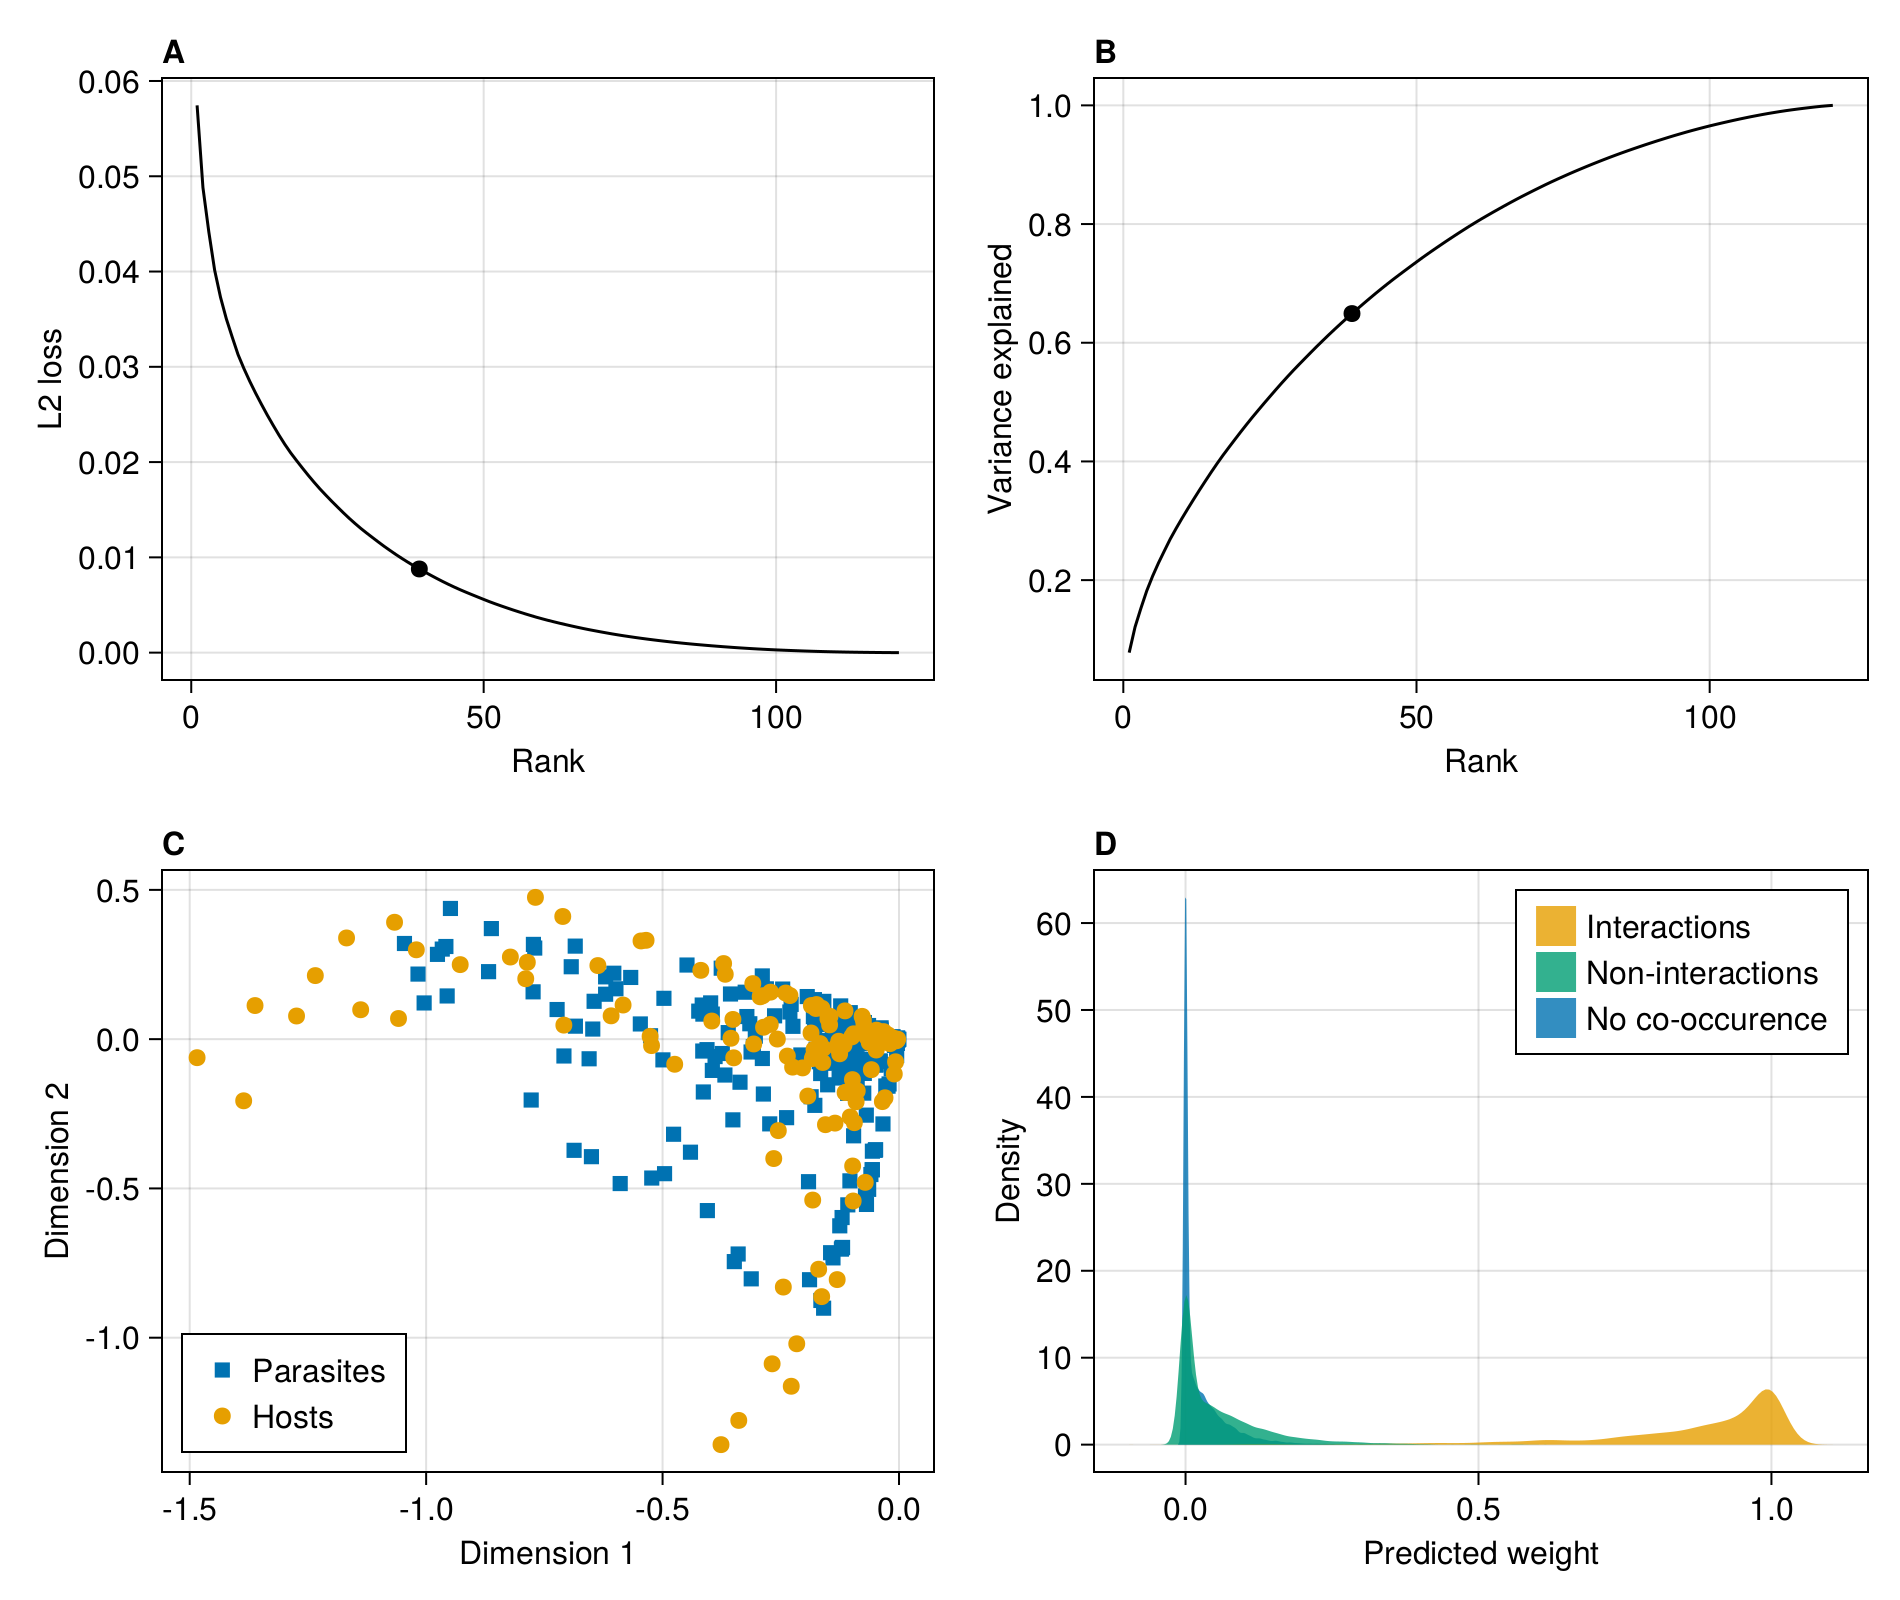
\includegraphics{index_files/figure-latex/fig-illustration-1-output-1.png}

}

\caption{\label{fig-illustration-1}Validation of an embedding for a
host-parasite metaweb, using Random Dot Product Graphs. \textbf{A},
decrease in approximation error as the number of dimensions in the
subspaces increases. \textbf{B}, increase in cumulative variance
explained as the number of ranks considered increases; in \textbf{A} and
\textbf{B}, the dot represents the point of inflexion in the curve (at
rank 39) estimated using the finite differences method. \textbf{C},
position of hosts and parasites in the space of latent variables on the
first and second dimensions of their respective subspaces (the results
have been clamped to the unit interval). \textbf{D}, predicted
interaction weight from the RDPG based on the status of the species pair
in the metaweb. Source:
\href{https://PoisotLab.github.io/ms_metaweb_perspectives/notebooks/SupplementaryMaterial-preview.html\#cell-fig-illustration-1}{Demonstration
of metaweb embedding using RDPG}}

\end{figure}

In Figure~\ref{fig-illustration-1}, we focus on some statistical checks
of the embedding. In panel \textbf{A}, we show that the averaged \(L_2\)
loss (\emph{i.e.} the mean of squared errors) between the empirical and
reconstructed metaweb decreases when the number of dimensions (rank) of
the subspace increases, with an inflection at 39 dimensions (out of 120
initially) according to the finite differences method. As discussed by
Runghen, Stouffer, and Dalla Riva (2021), there is often a trade-off
between the number of dimensions to use (more dimensions are more
computationally demanding) and the quality of the representation. In
panel \textbf{B}, we show the increase in cumulative variance explained
at each rank, and visualize that using 39 ranks explains about 70\% of
the variance in the empirical metaweb. This provides different
information from the \(L_2\) loss (which is averaged across
interactions), as it works on the eigenvalues of the embedding, and
therefore captures higher-level features of the network. In panel
\textbf{C}, we show positions of hosts and parasites on the first two
dimensions of the left and right subspaces. Note that these values
largely skew negative, because the first dimensions capture the coarse
structure of the network: most pairs of species do not interact, and
therefore have negative values. Finally in panel \textbf{D}, we show the
predicted weight (\emph{i.e.} the result of the multiplication of the
RDGP subspaces at a rank of 39) as a function of whether the
interactions are observed, not-observed, or unknown due to lack of
co-occurrence in the original dataset. This reveals that the observed
interactions have higher predicted weights, although there is some
overlap; the usual approach to identify potential interactions based on
this information would be a thresholding analysis, which is outside the
scope of this manuscript (and is done in the papers cited in this
illustration). Because the values returned from RDPG are not bound to
the unit interval, we performed a clamping of the weights to the unit
space, showing a one-inflation in documented interactions, and a
zero-inflation in other species pairs. Panel \textbf{D} specifically
shows that species pairs with no documented co-occurrence have weights
that are not distinguishable from species pairs with no documented
interactions; in other words, looking at the embedding, species that do
not co-occur are not easily distinguished from species that do not
interact. This suggests that (as befits a host-parasite model) the
ability to interact is a strong predictor of co-occurrence.

\begin{figure}[H]

{\centering 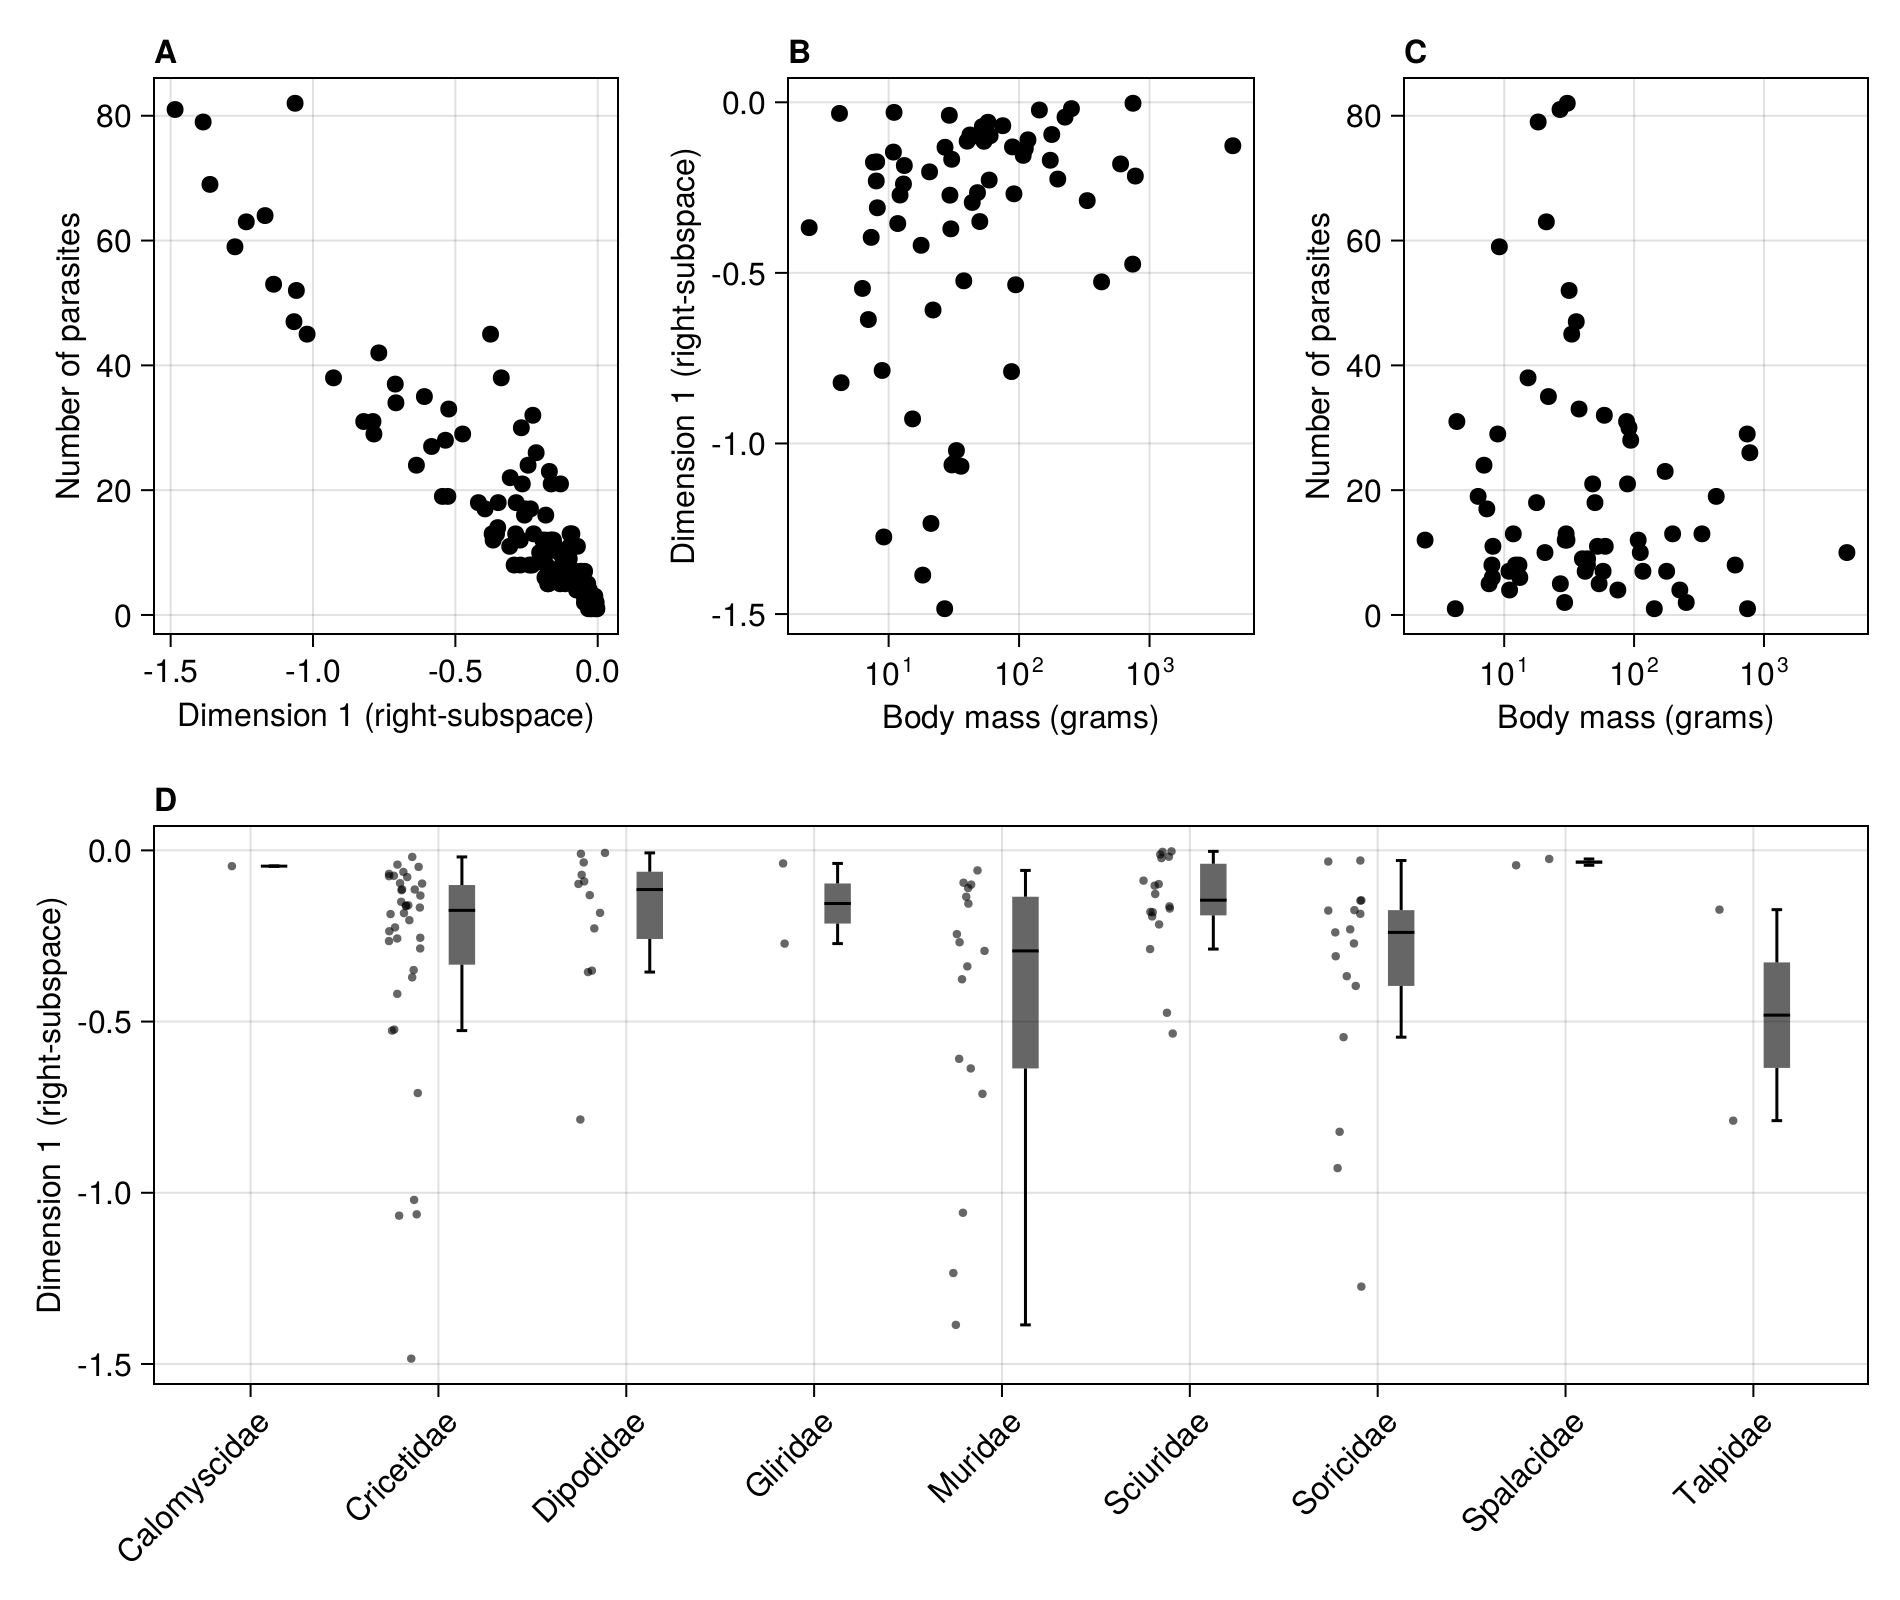
\includegraphics{index_files/figure-latex/fig-illustration-2-output-1.png}

}

\caption{\label{fig-illustration-2}Ecological analysis of an embedding
for a host-parasite metaweb, using Random Dot Product Graphs.
\textbf{A}, relationship between the number of parasites and position
along the first axis of the right-subspace for all hosts, showing that
the embedding captures elements of network structure at the species
scale. \textbf{B}, weak relationship between the body mass of hosts (in
grams) and the position alongside the same dimension. \textbf{C}, weak
relationship between body mass of hosts and parasite richness.
\textbf{D}, distribution of positions alongside the same axis for hosts
grouped by taxonomic family. Source:
\href{https://PoisotLab.github.io/ms_metaweb_perspectives/notebooks/SupplementaryMaterial-preview.html\#cell-fig-illustration-2}{Demonstration
of metaweb embedding using RDPG}}

\end{figure}

In Figure~\ref{fig-illustration-2}, we relate the values of latent
variables for hosts to different ecologically-relevant data; we can
perform this additional step, because the results presented in
Figure~\ref{fig-illustration-1} show that we can extract an embedding of
the metaweb that captures enough variance to be relevant. Importantly,
this is true for both \(L_2\) loss (indicating that RDPG is able to
capture pairwise processes) and the cumulative variance explained
(indicating that RDPG is able to capture network-level structure), which
suggests that these approaches may allow to predict interactions
\emph{and} network structure. In panel \textbf{A}, we show that host
with a higher value on the first dimension have fewer parasites. This
relates to the body size of hosts in the \emph{PanTHERIA} database
(Jones et al. 2009), as shown in panel \textbf{B}: interestingly, the
position on the first axis is only weakly correlated to body mass of the
host; this matches well established results showing that body size/mass
is not always a direct predictor of parasite richness in terrestrial
mammals (Morand and Poulin 1998), a result we observe in panel
\textbf{C}. Finally, in panel \textbf{D}, we can see how different
taxonomic families occupy different positions on the first axis, with
\emph{e.g.} Sciuridae being biased towards higher values. These results
show how we can look for ecological informations in the output of
network embeddings, which can further be refined into the selection of
predictors for transfer learning.

\hypertarget{the-metaweb-merges-ecological-hypotheses-and-practices}{%
\section{The metaweb merges ecological hypotheses and
practices}\label{the-metaweb-merges-ecological-hypotheses-and-practices}}

Metaweb inference seeks to provide information about the interactions
between species at a large spatial scale, typically a scale large enough
to be considered of biogeographic relevance (indeed, many of the
examples covered in the introduction span areas larger than a country,
some of them global). But as Herbert (1965) rightfully pointed out,
``{[}y{]}ou can't draw neat lines around planet-wide problems''; any
inference of a metaweb must therefore contend with several novel,
interwoven, families of problems. In this section, we outline three that
we think are particularly important, and discuss how they may be
addressed with subsequent data analysis or simulations, and how they
emerge in the specific context of using embeddings; some of these issues
are related to the application of these methods at the science-policy
interface. Adressing these considerations as part of the methodological
discussion is particularly important, as the construction of metawebs
can perpetuate legacies of biases in data (Box 2).

\hypertarget{identifying-the-properties-of-the-network-to-embed}{%
\subsection{Identifying the properties of the network to
embed}\label{identifying-the-properties-of-the-network-to-embed}}

If the initial metaweb is too narrow in scope, notably from a taxonomic
point of view, the chances decrease of finding another area with enough
related species (through phylogenetic relatedness or similarity of
functional traits) to make a reliable inference. This is because
transfer requires similarity (Figure~\ref{fig-embedding}). A diagnostic
for the lack of similar species would likely be large confidence
intervals during estimation of the values in the low-rank space. In
other words, the representation of the original graph is difficult to
transfer to the new problem. Alternatively, if the initial metaweb is
too large (taxonomically), then the resulting embeddings would need to
represent interactions between taxonomic groups that are not present in
the new location. This would lead to a much higher variance in the
starting dataset, and to under-dispersion in the target dataset,
resulting in the potential under or over estimation of the strength of
new predicted interactions. Llewelyn et al. (2022) provided compelling
evidence for these situations by showing that, even at small spatial
scales, the transfer of information about interactions becomes more
challenging when areas rich with endemic species are considered. The
lack of well documented metawebs is currently preventing the development
of more concrete guidelines. The question of phylogenetic relatedness
and distribution is notably relevant if the metaweb is assembled in an
area with mostly endemic species (\emph{e.g.} a system that has
undergone recent radiation or that has remained in isolation for a long
period of time might not have an analogous system with which to draw
knowledge from), and as with every predictive algorithm, there is room
for the application of our best ecological judgement. Because this
problem relates to distribution of species in the geographic or
phylogenetic space, it can certainly be approached through assessing the
performance of embedding transfer in simulated starting/target species
pools.

\hypertarget{identifying-the-scope-of-the-prediction-to-perform}{%
\subsection{Identifying the scope of the prediction to
perform}\label{identifying-the-scope-of-the-prediction-to-perform}}

The area for which we seek to predict the metaweb should determine the
species pool on which the embedding is performed. Metawebs can be
constructed by assigning interactions in a list of species within
specific regions. The upside of this approach is that information
relevant for the construction of this dataset is likely to exist, as
countries usually set conservation goals at the national level (Buxton
et al. 2021), and as quantitative instruments are consequently designed
to work at these scales (Turak et al. 2017); specific strategies are
often enacted at smaller scales, nested within a specific country (Ray,
Grimm, and Olive 2021). However, there is no guarantee that these
arbitrary boundaries are meaningful. In fact, we do not have a
satisfying answer to the question of ``where does an ecological network
stop?'', the answer to which would dictate the spatial span to
embed/predict. Recent results by Martins et al. (2022) suggested that
networks are shaped within eco-regions, with abrupt structural
transitions from an eco-region to the next. Should this trend hold
generally, this would provide an ecologically-relevant scale at which
metawebs can be downscaled and predicted. Other solutions could leverage
network-area relationships to identify areas in which networks are
structurally similar (see \emph{e.g.} Fortin, Dale, and Brimacombe 2021;
Galiana et al. 2018, 2022). Both of these solutions require ample
pre-existing information about the network in space. Nevertheless, the
inclusion of species for which we have data but that are not in the
right spatial extent \emph{may} improve the performance of approaches
based on embedding and transfer, \emph{if} they increase the similarity
between the target and destination network. This proposal can
specifically be evaluated by adding nodes to the network to embed, and
assessing the performance of predictive models (see \emph{e.g.} Llewelyn
et al. 2022).

\hypertarget{putting-models-in-their-context}{%
\subsection{Putting models in their
context}\label{putting-models-in-their-context}}

Predictive approaches in ecology, regardless of the scale at which they
are deployed and the intent of their deployment, originate in the
framework that contributed to the ongoing biodiversity crisis (Adam
2014) and reinforced environmental injustice (Choudry 2013; Domínguez
and Luoma 2020). The risk of embedding this legacy in our models is
real, especially when the impact of this legacy on species pools is
being increasingly documented. This problem can be addressed by
re-framing the way we interact with models, especially when models are
intended to support conservation actions. Particularly on territories
that were traditionally stewarded by Indigenous people, we must
interrogate how predictive approaches and the biases that underpin them
can be put to task in accompanying Indigenous principles of land
management (Eichhorn, Baker, and Griffiths 2019; No'kmaq et al. 2021).
The discussion of ``algorithm-in-the-loop'' approaches that is now
pervasive in the machine learning community provides examples of why
this is important. Human-algorithm interactions are notoriously
difficult and can yield adverse effects (Green and Chen 2019; Stevenson
and Doleac 2021), suggesting the need to systematically study them for
the specific purpose of, here, biodiversity governance. Improving the
algorithmic literacy of decision makers is part of the solution
(\emph{e.g.} Lamba et al. 2019; Mosebo Fernandes et al. 2020), as we can
reasonably expect that model outputs will be increasingly used to drive
policy decisions (Weiskopf et al. 2022). Our discussion of these
approaches need to go beyond the technical and statistical, and into the
governance consequences they can have. To embed data also embeds
historical and contemporary biases that acted on these data, both
because they shaped the ecological processes generating them (see Box
2), and the global processes leading to their measurement and
publication. For a domain as vast as species interaction networks, these
biases exist at multiple scales along the way, and a challenge for
prediction is not only to develop (or adopt) new quantitative tools, but
to assess the behavior of these tools in the proper context.

\hypertarget{conclusion}{%
\section{Conclusion}\label{conclusion}}

Although promising, the application of embeddings to metaweb prediction
still involved several challenges. First, there is a need to understand
how to define a metaweb as a single, cohesive, unit of ecological
organisation. This is likely to have very different answers based on the
specific taxonomic group, temporal and spatial resolution, and question
being investigated. Second, there is a need to understand the scale at
which these predictions are relevant. Although we have documented many
cases of using embedding to fill gaps in the metaweb, these techniques
can likely be brought into a spatial (and possibly temporal) context.
The validation of these predictions will have to proceed jointly with
empirical sampling of interactions, but also with the design of
downsampling methods. Finally, there is a need for a greater
understanding of how biases in the data propagate to the predictions.
Because the volume of metawebs is currently low, and because graph
embeddings have not been commonly applied, we anticipate that this
discussion will take place organically in the coming years.

\begin{tcolorbox}[enhanced jigsaw, coltitle=black, title=\textcolor{quarto-callout-note-color}{\faInfo}\hspace{0.5em}{Box 2 - Minding legacies shaping ecological datasets}, bottomtitle=1mm, colback=white, breakable, colbacktitle=quarto-callout-note-color!10!white, opacityback=0, left=2mm, arc=.35mm, colframe=quarto-callout-note-color-frame, toptitle=1mm, leftrule=.75mm, rightrule=.15mm, titlerule=0mm, bottomrule=.15mm, toprule=.15mm, opacitybacktitle=0.6]

In large parts of the world, boundaries that delineate geographic
regions are a legacy of settler colonialism, which drives global
disparity in capacity to collect and publish ecological data. Applying
any embedding to biased data does not debias them, but rather embeds
these biases, propagating them to the models using embeddings to make
predictions. Furthermore, the use of ecological data itself is not an
apolitical act (Nost and Goldstein 2021): data infrastructures tend to
be designed to answer questions within national boundaries (therefore
placing contingencies on what is available to be embedded), their use
often drawing upon, and reinforcing, territorial statecraft (see
\emph{e.g.} Barrett 2005). As per Machen and Nost (2021), these biases
are particularly important to consider when knowledge generated
algorithmically is used to supplement or replace human decision-making,
especially for governance (\emph{e.g.} enacting conservation decisions
on the basis of model prediction). As information on networks is
increasingly leveraged for conservation actions (see \emph{e.g.} Eero et
al. 2021; Naman et al. 2022; Stier et al. 2017), the need to appraise
and correct biases that are unwittingly propagated to algorithms when
embedded from the original data is immense. These considerations are
even more urgent in the specific context of biodiversity data. Long-term
colonial legacies still shape taxonomic composition to this day (Lenzner
et al. 2022; Raja 2022), and much shorter-term changes in taxonomic and
genetic richness of wildlife emerged through environmental racism
(Schmidt and Garroway 2022). Thus, the set of species found at a
specific location is not only as the result of a response to ecological
processes separate from human influence, but also the result of
human-environment interaction as well as the results of
legislative/political histories.

\end{tcolorbox}

\textbf{Acknowledgements:} We acknowledge that this study was conducted
on land within the traditional unceded territory of the Saint Lawrence
Iroquoian, Anishinabewaki, Mohawk, Huron-Wendat, and Omàmiwininiwak
nations. We thank Victoria hemming for feedback on this manuscript. TP,
TS, DC, and LP received funding from the Canadian Institute for Ecology
\& Evolution. FB is funded by the Institute for Data Valorization
(IVADO). TS, SB, and TP are funded by a donation from the Courtois
Foundation. M-JF acknowledges funding from NSERC Discovery Grant and
NSERC CRC. RR is funded by New Zealand's Biological Heritage Ngā Koiora
Tuku Iho National Science Challenge, administered by New Zealand
Ministry of Business, Innovation, and Employment. BM is funded by the
NSERC Alexander Graham Bell Canada Graduate Scholarship and the FRQNT
master's scholarship. LP acknowledges funding from NSERC Discovery Grant
(NSERC RGPIN-2019-05771). TP acknowledges financial support from the
Fondation Courtois, and NSERC through the Discovery Grants and Discovery
Accelerator Supplement programs. MJF is supported by an NSERC PDF and an
RBC Post-Doctoral Fellowship.

\textbf{Conflict of interest:} The authors have no conflict of interests
to disclose

\textbf{Authors' contributions:} TS and TP conceived the ideas discussed
in the manuscript. All authors contributed to writing and editing the
manuscript.

\textbf{Data availability:} The code to collect the data use in figures
is distributed as part of the Supplementary Material.

\hypertarget{references}{%
\section*{References}\label{references}}
\addcontentsline{toc}{section}{References}

\hypertarget{refs}{}
\begin{CSLReferences}{1}{0}
\leavevmode\vadjust pre{\hypertarget{ref-Adam2014Elephant}{}}%
Adam, Rachelle. 2014. \emph{Elephant Treaties: {The Colonial} Legacy of
the Biodiversity Crisis}. {UPNE}.

\leavevmode\vadjust pre{\hypertarget{ref-Albouy2019Marine}{}}%
Albouy, Camille, Philippe Archambault, Ward Appeltans, Miguel B. Araújo,
David Beauchesne, Kevin Cazelles, Alyssa R. Cirtwill, et al. 2019.
{``The Marine Fish Food Web Is Globally Connected.''} \emph{Nature
Ecology \& Evolution} 3 (8, 8): 1153--61.
\url{https://doi.org/10.1038/s41559-019-0950-y}.

\leavevmode\vadjust pre{\hypertarget{ref-Anowar2021Conceptual}{}}%
Anowar, Farzana, Samira Sadaoui, and Bassant Selim. 2021. {``Conceptual
and Empirical Comparison of Dimensionality Reduction Algorithms ({PCA},
{KPCA}, {LDA}, {MDS}, {SVD}, {LLE}, {ISOMAP}, {LE}, {ICA}, t-{SNE}).''}
\emph{Computer Science Review} 40 (May): 100378.
\url{https://doi.org/10.1016/j.cosrev.2021.100378}.

\leavevmode\vadjust pre{\hypertarget{ref-Arsov2019Network}{}}%
Arsov, Nino, and Georgina Mirceva. 2019. {``Network {Embedding}: {An
Overview}.''} \url{http://arxiv.org/abs/1911.11726}.

\leavevmode\vadjust pre{\hypertarget{ref-Athreya2017Statistical}{}}%
Athreya, Avanti, Donniell E. Fishkind, Keith Levin, Vince Lyzinski,
Youngser Park, Yichen Qin, Daniel L. Sussman, Minh Tang, Joshua T.
Vogelstein, and Carey E. Priebe. 2017. {``Statistical Inference on
Random Dot Product Graphs: A Survey.''} {arXiv}.
\url{http://arxiv.org/abs/1709.05454}.

\leavevmode\vadjust pre{\hypertarget{ref-Barrett2005Environment}{}}%
Barrett, Scott. 2005. \emph{Environment and {Statecraft}: {The Strategy}
of {Environmental Treaty-Making}}. 1st ed. {Oxford University
PressOxford}. \url{https://doi.org/10.1093/0199286094.001.0001}.

\leavevmode\vadjust pre{\hypertarget{ref-Bartomeus2013Understanding}{}}%
Bartomeus, Ignasi. 2013. {``Understanding Linkage Rules in
Plant-Pollinator Networks by Using Hierarchical Models That Incorporate
Pollinator Detectability and Plant Traits.''} \emph{PloS One} 8 (7):
e69200.
\url{http://journals.plos.org/plosone/article?id=10.1371/journal.pone.0069200}.

\leavevmode\vadjust pre{\hypertarget{ref-Bartomeus2016Common}{}}%
Bartomeus, Ignasi, Dominique Gravel, Jason M. Tylianakis, Marcelo A.
Aizen, Ian A. Dickie, and Maud Bernard-Verdier. 2016. {``A Common
Framework for Identifying Linkage Rules Across Different Types of
Interactions.''} \emph{Functional Ecology} 30 (12): 1894--1903.
\url{http://onlinelibrary.wiley.com/doi/10.1111/1365-2435.12666/full}.

\leavevmode\vadjust pre{\hypertarget{ref-Bezanson2017Julia}{}}%
Bezanson, Jeff, Alan Edelman, Stefan Karpinski, and Viral B. Shah. 2017.
{``Julia: {A Fresh Approach} to {Numerical Computing}.''} \emph{SIAM
Review} 59 (1): 65--98. \url{https://doi.org/10.1137/141000671}.

\leavevmode\vadjust pre{\hypertarget{ref-Blanchet2020Cooccurrence}{}}%
Blanchet, F. Guillaume, Kevin Cazelles, and Dominique Gravel. 2020.
{``Co-Occurrence Is Not Evidence of Ecological Interactions.''}
\emph{Ecology Letters}.

\leavevmode\vadjust pre{\hypertarget{ref-Bohan2017Nextgeneration}{}}%
Bohan, David A., Corinne Vacher, Alireza Tamaddoni-Nezhad, Alan
Raybould, Alex J. Dumbrell, and Guy Woodward. 2017. {``Next-{Generation
Global Biomonitoring}: {Large-scale}, {Automated Reconstruction} of
{Ecological Networks}.''} \emph{Trends in Ecology \& Evolution}, March.
\url{https://doi.org/10.1016/j.tree.2017.03.001}.

\leavevmode\vadjust pre{\hypertarget{ref-Botella2022Appraisal}{}}%
Botella, Christophe, Stéphane Dray, Catherine Matias, Vincent Miele, and
Wilfried Thuiller. 2022. {``An Appraisal of Graph Embeddings for
Comparing Trophic Network Architectures.''} \emph{Methods in Ecology and
Evolution} 13 (1): 203--16.
\url{https://doi.org/10.1111/2041-210X.13738}.

\leavevmode\vadjust pre{\hypertarget{ref-Braga2019Spatial}{}}%
Braga, João, Laura J. Pollock, Ceres Barros, Núria Galiana, José M.
Montoya, Dominique Gravel, Luigi Maiorano, et al. 2019. {``Spatial
Analyses of Multi-Trophic Terrestrial Vertebrate Assemblages in
{Europe}.''} \emph{Global Ecology and Biogeography} 28 (11): 1636--48.
\url{https://doi.org/10.1111/geb.12981}.

\leavevmode\vadjust pre{\hypertarget{ref-Braga2021Phylogenetic}{}}%
Braga, Mariana P., Niklas Janz, Sören Nylin, Fredrik Ronquist, and
Michael J. Landis. 2021. {``Phylogenetic Reconstruction of Ancestral
Ecological Networks Through Time for Pierid Butterflies and Their Host
Plants.''} \emph{Ecology Letters} n/a (n/a).
\url{https://doi.org/10.1111/ele.13842}.

\leavevmode\vadjust pre{\hypertarget{ref-BramonMora2018Identifying}{}}%
Bramon Mora, Bernat, Dominique Gravel, Luis J. Gilarranz, Timothée
Poisot, and Daniel B. Stouffer. 2018. {``Identifying a Common Backbone
of Interactions Underlying Food Webs from Different Ecosystems.''}
\emph{Nature Communications} 9 (1): 2603.
\url{https://doi.org/10.1038/s41467-018-05056-0}.

\leavevmode\vadjust pre{\hypertarget{ref-Buxton2021Key}{}}%
Buxton, Rachel T., Joseph R. Bennett, Andrea J. Reid, Charles Shulman,
Steven J. Cooke, Charles M. Francis, Elizabeth A. Nyboer, et al. 2021.
{``Key Information Needs to Move from Knowledge to Action for
Biodiversity Conservation in {Canada}.''} \emph{Biological Conservation}
256 (April): 108983. \url{https://doi.org/10.1016/j.biocon.2021.108983}.

\leavevmode\vadjust pre{\hypertarget{ref-carlson2022}{}}%
Carlson, Colin J., Gregory F. Albery, Cory Merow, Christopher H. Trisos,
Casey M. Zipfel, Evan A. Eskew, Kevin J. Olival, Noam Ross, and Shweta
Bansal. 2022. {``Climate Change Increases Cross-Species Viral
Transmission Risk.''} \emph{Nature} 607 (7919): 555--62.
\url{https://doi.org/10.1038/s41586-022-04788-w}.

\leavevmode\vadjust pre{\hypertarget{ref-Catchen2023Missing}{}}%
Catchen, Michael, Timothée Poisot, Laura Pollock, and Andrew Gonzalez.
2023. {``The Missing Link: Discerning True from False Negatives When
Sampling Species Interaction Networks.''} Preprint. {EcoEvoRXiV}.
\url{https://doi.org/10.32942/X2DW22}.

\leavevmode\vadjust pre{\hypertarget{ref-Cazelles2016Theory}{}}%
Cazelles, Kévin, Miguel B. Araújo, Nicolas Mouquet, and Dominique
Gravel. 2016. {``A Theory for Species Co-Occurrence in Interaction
Networks.''} \emph{Theoretical Ecology} 9 (1): 39--48.
\url{https://doi.org/10.1007/s12080-015-0281-9}.

\leavevmode\vadjust pre{\hypertarget{ref-Chami2022Machine}{}}%
Chami, Ines, Sami Abu-El-Haija, Bryan Perozzi, Christopher Ré, and Kevin
Murphy. 2022. {``Machine {Learning} on {Graphs}: {A Model} and
{Comprehensive Taxonomy}.''} \emph{Journal of Machine Learning Research}
23 (89): 1--64. \url{http://jmlr.org/papers/v23/20-852.html}.

\leavevmode\vadjust pre{\hypertarget{ref-Chen2017Deep}{}}%
Chen, Di, Yexiang Xue, Daniel Fink, Shuo Chen, and Carla P. Gomes. 2017.
{``Deep {Multi-species Embedding},''} 3639--46.
\url{https://www.ijcai.org/proceedings/2017/509}.

\leavevmode\vadjust pre{\hypertarget{ref-Chen2017Harp}{}}%
Chen, Haochen, Bryan Perozzi, Yifan Hu, and Steven Skiena. 2017.
{``{HARP}: {Hierarchical Representation Learning} for {Networks}.''}
\url{http://arxiv.org/abs/1706.07845}.

\leavevmode\vadjust pre{\hypertarget{ref-Choudry2013Saving}{}}%
Choudry, Aziz. 2013. {``Saving Biodiversity, for Whom and for What?
{Conservation NGOs}, Complicity, Colonialism and Conquest in an Era of
Capitalist Globalization.''} In \emph{{NGOization}: {Complicity},
Contradictions and Prospects}, 24--44. {Bloomsbury Publishing}.

\leavevmode\vadjust pre{\hypertarget{ref-Cieslak2020Tdistributed}{}}%
Cieslak, Matthew C., Ann M. Castelfranco, Vittoria Roncalli, Petra H.
Lenz, and Daniel K. Hartline. 2020. {``T-{Distributed Stochastic
Neighbor Embedding} (t-{SNE}): {A} Tool for Eco-Physiological
Transcriptomic Analysis.''} \emph{Marine Genomics} 51 (June): 100723.
\url{https://doi.org/10.1016/j.margen.2019.100723}.

\leavevmode\vadjust pre{\hypertarget{ref-Csermely2004Strong}{}}%
Csermely, Peter. 2004. {``Strong Links Are Important, but Weak Links
Stabilize Them.''} \emph{Trends in Biochemical Sciences} 29 (7):
331--34. \url{https://doi.org/10.1016/j.tibs.2004.05.004}.

\leavevmode\vadjust pre{\hypertarget{ref-DallaRiva2016Exploring}{}}%
Dalla Riva, Giulio V., and Daniel B. Stouffer. 2016. {``Exploring the
Evolutionary Signature of Food Webs' Backbones Using Functional
Traits.''} \emph{Oikos} 125 (4): 446--56.
\url{https://doi.org/10.1111/oik.02305}.

\leavevmode\vadjust pre{\hypertarget{ref-Dallas2017Predicting}{}}%
Dallas, Tad, Andrew W. Park, and John M. Drake. 2017. {``Predicting
Cryptic Links in Host-Parasite Networks.''} \emph{PLOS Computational
Biology} 13 (5): e1005557.
\url{https://doi.org/10.1371/journal.pcbi.1005557}.

\leavevmode\vadjust pre{\hypertarget{ref-Danisch2021Makie}{}}%
Danisch, Simon, and Julius Krumbiegel. 2021. {``Makie.jl: {Flexible}
High-Performance Data Visualization for {Julia}.''} \emph{Journal of
Open Source Software} 6 (65): 3349.
\url{https://doi.org/10.21105/joss.03349}.

\leavevmode\vadjust pre{\hypertarget{ref-Dominguez2020Decolonising}{}}%
Domínguez, Lara, and Colin Luoma. 2020. {``Decolonising {Conservation
Policy}: {How Colonial Land} and {Conservation Ideologies Persist} and
{Perpetuate Indigenous Injustices} at the {Expense} of the
{Environment}.''} \emph{Land} 9 (3, 3): 65.
\url{https://doi.org/10.3390/land9030065}.

\leavevmode\vadjust pre{\hypertarget{ref-Dunne2006Network}{}}%
Dunne, Jennifer A. 2006. {``The {Network Structure} of {Food Webs}.''}
In \emph{Ecological Networks: {Linking} Structure and Dynamics}, edited
by Jennifer A Dunne and Mercedes Pascual, 27--86. {Oxford University
Press}.

\leavevmode\vadjust pre{\hypertarget{ref-Eero2021Use}{}}%
Eero, Margit, Jan Dierking, Christoph Humborg, Emma Undeman, Brian R
MacKenzie, Henn Ojaveer, Tiina Salo, and Friedrich Wilhelm Köster. 2021.
{``Use of Food Web Knowledge in Environmental Conservation and
Management of Living Resources in the {Baltic Sea}.''} \emph{ICES
Journal of Marine Science} 78 (8): 2645--63.
\url{https://doi.org/10.1093/icesjms/fsab145}.

\leavevmode\vadjust pre{\hypertarget{ref-Eichhorn2019Steps}{}}%
Eichhorn, Markus P., Kate Baker, and Mark Griffiths. 2019. {``Steps
Towards Decolonising Biogeography.''} \emph{Frontiers of Biogeography}
12 (1): 1--7. \url{https://doi.org/10.21425/F5FBG44795}.

\leavevmode\vadjust pre{\hypertarget{ref-Eklof2013Dimensionality}{}}%
Eklöf, Anna, Ute Jacob, Jason Kopp, Jordi Bosch, Rocío Castro-Urgal,
Natacha P. Chacoff, Bo Dalsgaard, et al. 2013. {``The Dimensionality of
Ecological Networks.''} \emph{Ecology Letters} 16 (5): 577--83.
\url{https://doi.org/10.1111/ele.12081}.

\leavevmode\vadjust pre{\hypertarget{ref-Eklof2016Phylogenetic}{}}%
Eklöf, Anna, and Daniel B. Stouffer. 2016. {``The Phylogenetic Component
of Food Web Structure and Intervality.''} \emph{Theoretical Ecology} 9
(1): 107--15. \url{https://doi.org/10.1007/s12080-015-0273-9}.

\leavevmode\vadjust pre{\hypertarget{ref-Fortin2021Network}{}}%
Fortin, Marie-Josée, Mark R. T. Dale, and Chris Brimacombe. 2021.
{``Network Ecology in Dynamic Landscapes.''} \emph{Proceedings of the
Royal Society B: Biological Sciences} 288 (1949): rspb.2020.1889,
20201889. \url{https://doi.org/10.1098/rspb.2020.1889}.

\leavevmode\vadjust pre{\hypertarget{ref-Fricke2022Effects}{}}%
Fricke, Evan C., Alejandro Ordonez, Haldre S. Rogers, and Jens-Christian
Svenning. 2022. {``The Effects of Defaunation on Plants' Capacity to
Track Climate Change.''} \emph{Science}, January.
\url{https://www.science.org/doi/abs/10.1126/science.abk3510}.

\leavevmode\vadjust pre{\hypertarget{ref-Galiana2022Ecological}{}}%
Galiana, Núria, Miguel Lurgi, Vinicius A. G. Bastazini, Jordi Bosch,
Luciano Cagnolo, Kevin Cazelles, Bernat Claramunt-López, et al. 2022.
{``Ecological Network Complexity Scales with Area.''} \emph{Nature
Ecology \& Evolution}, January, 1--8.
\url{https://doi.org/10.1038/s41559-021-01644-4}.

\leavevmode\vadjust pre{\hypertarget{ref-Galiana2018Spatial}{}}%
Galiana, Núria, Miguel Lurgi, Bernat Claramunt-López, Marie-Josée
Fortin, Shawn Leroux, Kevin Cazelles, Dominique Gravel, and José M.
Montoya. 2018. {``The Spatial Scaling of Species Interaction
Networks.''} \emph{Nature Ecology \& Evolution} 2 (5): 782--90.
\url{https://doi.org/10.1038/s41559-018-0517-3}.

\leavevmode\vadjust pre{\hypertarget{ref-Gaucher2021Outlier}{}}%
Gaucher, Solenne, Olga Klopp, and Geneviève Robin. 2021. {``Outlier
Detection in Networks with Missing Links.''} \emph{Computational
Statistics \& Data Analysis} 164 (December): 107308.
\url{https://doi.org/10.1016/j.csda.2021.107308}.

\leavevmode\vadjust pre{\hypertarget{ref-ghasemian2020}{}}%
Ghasemian, Amir, Homa Hosseinmardi, Aram Galstyan, Edoardo M. Airoldi,
and Aaron Clauset. 2020. {``Stacking Models for Nearly Optimal Link
Prediction in Complex Networks.''} \emph{Proceedings of the National
Academy of Sciences} 117 (38): 23393--400.
\url{https://doi.org/10.1073/pnas.1914950117}.

\leavevmode\vadjust pre{\hypertarget{ref-Gibb2021Data}{}}%
Gibb, Rory, Gregory F Albery, Daniel J Becker, Liam Brierley, Ryan
Connor, Tad A Dallas, Evan A Eskew, et al. 2021. {``Data
{Proliferation}, {Reconciliation}, and {Synthesis} in {Viral
Ecology}.''} \emph{BioScience} 71 (11): 1148--56.
\url{https://doi.org/10.1093/biosci/biab080}.

\leavevmode\vadjust pre{\hypertarget{ref-Goebel2023Body}{}}%
Goebel, Larissa Gabriela Araujo, Breno Dias Vitorino, Angélica Vilas
Boas Frota, and Manoel dos Santos-Filho. 2023. {``Body Mass Determines
the Role of Mammal Species in a Frugivore-Large Fruit Interaction
Network in a {Neotropical} Savanna.''} \emph{Journal of Tropical
Ecology} 39: e12. \url{https://doi.org/10.1017/S0266467422000505}.

\leavevmode\vadjust pre{\hypertarget{ref-Goodfellow2016Deep}{}}%
Goodfellow, Ian, Yoshua Bengio, and Aaron Courville. 2016. \emph{Deep
Learning}. {MIT Press}.

\leavevmode\vadjust pre{\hypertarget{ref-Goyal2018Graph}{}}%
Goyal, Palash, and Emilio Ferrara. 2018. {``Graph Embedding Techniques,
Applications, and Performance: {A} Survey.''} \emph{Knowledge-Based
Systems} 151 (July): 78--94.
\url{https://doi.org/10.1016/j.knosys.2018.03.022}.

\leavevmode\vadjust pre{\hypertarget{ref-Gravel2018Bringing}{}}%
Gravel, Dominique, Benjamin Baiser, Jennifer A. Dunne, Jens-Peter
Kopelke, Neo D. Martinez, Tommi Nyman, Timothée Poisot, et al. 2018.
{``Bringing {Elton} and {Grinnell} Together: A Quantitative Framework to
Represent the Biogeography of Ecological Interaction Networks.''}
\emph{Ecography} 0 (0). \url{https://doi.org/10.1111/ecog.04006}.

\leavevmode\vadjust pre{\hypertarget{ref-Gravel2013Inferring}{}}%
Gravel, Dominique, Timothée Poisot, Camille Albouy, Laure Velez, and
David Mouillot. 2013. {``Inferring Food Web Structure from Predator-Prey
Body Size Relationships.''} Edited by Robert Freckleton. \emph{Methods
in Ecology and Evolution} 4 (11): 1083--90.
\url{https://doi.org/10.1111/2041-210X.12103}.

\leavevmode\vadjust pre{\hypertarget{ref-Green2019Disparate}{}}%
Green, Ben, and Yiling Chen. 2019. {``Disparate {Interactions}: {An
Algorithm-in-the-Loop Analysis} of {Fairness} in {Risk Assessments}.''}
In \emph{Proceedings of the {Conference} on {Fairness},
{Accountability}, and {Transparency}}, 90--99. {FAT}* '19. {New York,
NY, USA}: {Association for Computing Machinery}.
\url{https://doi.org/10.1145/3287560.3287563}.

\leavevmode\vadjust pre{\hypertarget{ref-Grover2016Node2vec}{}}%
Grover, Aditya, and Jure Leskovec. 2016. {``Node2vec: {Scalable Feature
Learning} for {Networks}.''} In \emph{Proceedings of the 22nd {ACM
SIGKDD International Conference} on {Knowledge Discovery} and {Data
Mining}}, 855--64. {San Francisco California USA}: {ACM}.
\url{https://doi.org/10.1145/2939672.2939754}.

\leavevmode\vadjust pre{\hypertarget{ref-Grunig2020Crop}{}}%
Grünig, Marc, Dominique Mazzi, Pierluigi Calanca, Dirk Nikolaus Karger,
and Loïc Pellissier. 2020. {``Crop and Forest Pest Metawebs Shift
Towards Increased Linkage and Suitability Overlap Under Climate
Change.''} \emph{Communications Biology} 3 (1, 1): 1--10.
\url{https://doi.org/10.1038/s42003-020-0962-9}.

\leavevmode\vadjust pre{\hypertarget{ref-Gupta2022Simultaneously}{}}%
Gupta, Anubhav, Reinhard Furrer, and Owen L. Petchey. 2022.
{``Simultaneously Estimating Food Web Connectance and Structure with
Uncertainty.''} \emph{Ecology and Evolution} 12 (3): e8643.
\url{https://doi.org/10.1002/ece3.8643}.

\leavevmode\vadjust pre{\hypertarget{ref-Gupta2021Graph}{}}%
Gupta, Atika, Priya Matta, and Bhasker Pant. 2021. {``Graph Neural
Network: {Current} State of {Art}, Challenges and Applications.''}
\emph{Materials Today: Proceedings}, International {Conference} on
{Technological Advancements} in {Materials Science} and {Manufacturing},
46 (January): 10927--32.
\url{https://doi.org/10.1016/j.matpr.2021.01.950}.

\leavevmode\vadjust pre{\hypertarget{ref-Hadfield2014Tale}{}}%
Hadfield, Jarrod D., Boris R. Krasnov, Robert Poulin, and Shinichi
Nakagawa. 2014. {``A {Tale} of {Two Phylogenies}: {Comparative Analyses}
of {Ecological Interactions}.''} \emph{The American Naturalist} 183 (2):
174--87. \url{https://doi.org/10.1086/674445}.

\leavevmode\vadjust pre{\hypertarget{ref-Herbert1965Dune}{}}%
Herbert, Frank. 1965. \emph{Dune}. 1st ed. {Philadelphia}: {Chilton Book
Company}.

\leavevmode\vadjust pre{\hypertarget{ref-Hinton2002Stochastic}{}}%
Hinton, Geoffrey, and Sam T Roweis. 2002. {``Stochastic Neighbor
Embedding.''} In \emph{{NIPS}}, 15:833--40. {Citeseer}.

\leavevmode\vadjust pre{\hypertarget{ref-Hoffmann2019Machine}{}}%
Hoffmann, Jordan, Yohai Bar-Sinai, Lisa M. Lee, Jovana Andrejevic,
Shruti Mishra, Shmuel M. Rubinstein, and Chris H. Rycroft. 2019.
{``Machine Learning in a Data-Limited Regime: {Augmenting} Experiments
with Synthetic Data Uncovers Order in Crumpled Sheets.''} \emph{Science
Advances} 5 (4): eaau6792. \url{https://doi.org/10.1126/sciadv.aau6792}.

\leavevmode\vadjust pre{\hypertarget{ref-Hortal2015Seven}{}}%
Hortal, Joaquín, Francesco de Bello, José Alexandre F. Diniz-Filho,
Thomas M. Lewinsohn, Jorge M. Lobo, and Richard J. Ladle. 2015. {``Seven
{Shortfalls} That {Beset Large-Scale Knowledge} of {Biodiversity}.''}
\emph{Annual Review of Ecology, Evolution, and Systematics} 46 (1):
523--49. \url{https://doi.org/10.1146/annurev-ecolsys-112414-054400}.

\leavevmode\vadjust pre{\hypertarget{ref-Jones2009Pantheria}{}}%
Jones, Kate E., Jon Bielby, Marcel Cardillo, Susanne A. Fritz, Justin
O'Dell, C. David L. Orme, Kamran Safi, et al. 2009. {``{PanTHERIA}: A
Species‐level Database of Life History, Ecology, and Geography of Extant
and Recently Extinct Mammals: {Ecological Archives E090}‐184.''} Edited
by W. K. Michener. \emph{Ecology} 90 (9): 2648--48.
\url{https://doi.org/10.1890/08-1494.1}.

\leavevmode\vadjust pre{\hypertarget{ref-Jordano2016Sampling}{}}%
Jordano, Pedro. 2016. {``Sampling Networks of Ecological
Interactions.''} Edited by Daniel Stouffer. \emph{Functional Ecology} 30
(12): 1883--93. \url{https://doi.org/10.1111/1365-2435.12763}.

\leavevmode\vadjust pre{\hypertarget{ref-Lamba2019Deep}{}}%
Lamba, Aakash, Phillip Cassey, Ramesh Raja Segaran, and Lian Pin Koh.
2019. {``Deep Learning for Environmental Conservation.''} \emph{Current
Biology} 29 (19): R977--82.
\url{https://doi.org/10.1016/j.cub.2019.08.016}.

\leavevmode\vadjust pre{\hypertarget{ref-Lenzner2022Naturalized}{}}%
Lenzner, Bernd, Guillaume Latombe, Anna Schertler, Hanno Seebens, Qiang
Yang, Marten Winter, Patrick Weigelt, et al. 2022. {``Naturalized Alien
Floras Still Carry the Legacy of {European} Colonialism.''} \emph{Nature
Ecology \& Evolution}, October, 1--10.
\url{https://doi.org/10.1038/s41559-022-01865-1}.

\leavevmode\vadjust pre{\hypertarget{ref-Llewelyn2022Predicting}{}}%
Llewelyn, John, Giovanni Strona, Christopher R. Dickman, Aaron C.
Greenville, Glenda M. Wardle, Michael S. Y. Lee, Seamus Doherty, Farzin
Shabani, Frédérik Saltré, and Corey J. A. Bradshaw. 2022. {``Predicting
Predator-Prey Interactions in Terrestrial Endotherms Using Random
Forest.''} Preprint. {Ecology}.
\url{https://doi.org/10.1101/2022.09.02.506446}.

\leavevmode\vadjust pre{\hypertarget{ref-Maaten2009Learning}{}}%
Maaten, Laurens van der. 2009. {``Learning a {Parametric Embedding} by
{Preserving Local Structure}.''} In \emph{Proceedings of the {Twelth
International Conference} on {Artificial Intelligence} and
{Statistics}}, 384--91. {PMLR}.
\url{https://proceedings.mlr.press/v5/maaten09a.html}.

\leavevmode\vadjust pre{\hypertarget{ref-Machen2021Thinking}{}}%
Machen, Ruth, and Eric Nost. 2021. {``Thinking Algorithmically: {The}
Making of Hegemonic Knowledge in Climate Governance.''}
\emph{Transactions of the Institute of British Geographers} 46 (3):
555--69. \url{https://doi.org/10.1111/tran.12441}.

\leavevmode\vadjust pre{\hypertarget{ref-Malaterre2019Functional}{}}%
Malaterre, Christophe, Antoine C Dussault, Ely Mermans, Gillian Barker,
Beatrix E Beisner, Frédéric Bouchard, Eric Desjardins, et al. 2019.
{``Functional {Diversity}: {An Epistemic Roadmap}.''} \emph{BioScience}
69 (10): 800--811. \url{https://doi.org/10.1093/biosci/biz089}.

\leavevmode\vadjust pre{\hypertarget{ref-Martins2022Global}{}}%
Martins, Lucas P., Daniel B. Stouffer, Pedro G. Blendinger, Katrin
Böhning-Gaese, Galo Buitrón-Jurado, Marta Correia, José Miguel Costa, et
al. 2022. {``Global and Regional Ecological Boundaries Explain Abrupt
Spatial Discontinuities in Avian Frugivory Interactions.''} \emph{Nature
Communications} 13 (1, 1): 6943.
\url{https://doi.org/10.1038/s41467-022-34355-w}.

\leavevmode\vadjust pre{\hypertarget{ref-McLeod2021Sampling}{}}%
McLeod, Anne, Shawn J. Leroux, Dominique Gravel, Cindy Chu, Alyssa R.
Cirtwill, Marie-Josée Fortin, Núria Galiana, Timothée Poisot, and
Spencer A. Wood. 2021. {``Sampling and Asymptotic Network Properties of
Spatial Multi-Trophic Networks.''} \emph{Oikos} n/a (n/a).
\url{https://doi.org/10.1111/oik.08650}.

\leavevmode\vadjust pre{\hypertarget{ref-Melnyk2020Graphkke}{}}%
Melnyk, Kateryna, Stefan Klus, Grégoire Montavon, and Tim O. F. Conrad.
2020. {``{GraphKKE}: Graph {Kernel Koopman} Embedding for Human
Microbiome Analysis.''} \emph{Applied Network Science} 5 (1): 96.
\url{https://doi.org/10.1007/s41109-020-00339-2}.

\leavevmode\vadjust pre{\hypertarget{ref-Morales-Castilla2015Inferring}{}}%
Morales-Castilla, Ignacio, Miguel G. Matias, Dominique Gravel, and
Miguel B. Araújo. 2015. {``Inferring Biotic Interactions from
Proxies.''} \emph{Trends in Ecology \& Evolution} 30 (6): 347--56.
\url{https://doi.org/10.1016/j.tree.2015.03.014}.

\leavevmode\vadjust pre{\hypertarget{ref-morales-castilla2021}{}}%
Morales-Castilla, Ignacio, Paula Pappalardo, Maxwell J. Farrell, A.
Alonso Aguirre, Shan Huang, Alyssa-Lois M. Gehman, Tad Dallas, Dominique
Gravel, and T. Jonathan Davies. 2021. {``Forecasting Parasite Sharing
Under Climate Change.''} \emph{Philosophical Transactions of the Royal
Society B: Biological Sciences} 376 (1837): 20200360.
\url{https://doi.org/10.1098/rstb.2020.0360}.

\leavevmode\vadjust pre{\hypertarget{ref-Morand1998Density}{}}%
Morand, Serge, and Robert Poulin. 1998. {``Density, Body Mass and
Parasite Species Richness of Terrestrial Mammals.''} \emph{Evolutionary
Ecology} 12 (6): 717--27. \url{https://doi.org/10.1023/A:1006537600093}.

\leavevmode\vadjust pre{\hypertarget{ref-MoseboFernandes2020Machine}{}}%
Mosebo Fernandes, Ana Cristina, Rebeca Quintero Gonzalez, Marie Ann
Lenihan-Clarke, Ezra Francis Leslie Trotter, and Jamal Jokar Arsanjani.
2020. {``Machine {Learning} for {Conservation Planning} in a {Changing
Climate}.''} \emph{Sustainability} 12 (18, 18): 7657.
\url{https://doi.org/10.3390/su12187657}.

\leavevmode\vadjust pre{\hypertarget{ref-Murphy2022Probabilistic}{}}%
Murphy, Kevin P. 2022. \emph{Probabilistic Machine Learning: {An}
Introduction}. {MIT Press}. \href{https://probml.ai}{probml.ai}.

\leavevmode\vadjust pre{\hypertarget{ref-Naman2022Food}{}}%
Naman, Sean M., Seth M. White, J. Ryan Bellmore, Peter A. McHugh,
Matthew J. Kaylor, Colden V. Baxter, Robert J. Danehy, Robert J. Naiman,
and Amy L. Puls. 2022. {``Food Web Perspectives and Methods for Riverine
Fish Conservation.''} \emph{WIREs Water} n/a (n/a): e1590.
\url{https://doi.org/10.1002/wat2.1590}.

\leavevmode\vadjust pre{\hypertarget{ref-Narayanan2017Graph2vec}{}}%
Narayanan, Annamalai, Mahinthan Chandramohan, Rajasekar Venkatesan,
Lihui Chen, Yang Liu, and Shantanu Jaiswal. 2017. {``Graph2vec:
{Learning Distributed Representations} of {Graphs}.''}
\url{http://arxiv.org/abs/1707.05005}.

\leavevmode\vadjust pre{\hypertarget{ref-Neutel2002Stability}{}}%
Neutel, Anje-Margriet, Johan A. P. Heesterbeek, and Peter C. de Ruiter.
2002. {``Stability in {Real Food Webs}: {Weak Links} in {Long Loops}.''}
\emph{Science} 296 (5570): 1120--23.
\url{https://doi.org/10.1126/science.1068326}.

\leavevmode\vadjust pre{\hypertarget{ref-Nokmaq2021Awakening}{}}%
No'kmaq, M'sit, Albert Marshall, Karen F. Beazley, Jessica Hum, shalan
joudry, Anastasia Papadopoulos, Sherry Pictou, Janet Rabesca, Lisa
Young, and Melanie Zurba. 2021. {``{`{Awakening} the Sleeping Giant'}:
Re-{Indigenization} Principles for Transforming Biodiversity
Conservation in {Canada} and Beyond.''} \emph{FACETS} 6 (1): 839--69.

\leavevmode\vadjust pre{\hypertarget{ref-Nost2021Political}{}}%
Nost, Eric, and Jenny Elaine Goldstein. 2021. {``A Political Ecology of
Data.''} \emph{Environment and Planning E: Nature and Space}, September,
25148486211043503. \url{https://doi.org/10.1177/25148486211043503}.

\leavevmode\vadjust pre{\hypertarget{ref-OConnor2020Unveiling}{}}%
O'Connor, Louise M. J., Laura J. Pollock, João Braga, Gentile Francesco
Ficetola, Luigi Maiorano, Camille Martinez‐Almoyna, Alessandro
Montemaggiori, Marc Ohlmann, and Wilfried Thuiller. 2020. {``Unveiling
the Food Webs of Tetrapods Across {Europe} Through the Prism of the
{Eltonian} Niche.''} \emph{Journal of Biogeography} 47 (1): 181--92.
\url{https://doi.org/10.1111/jbi.13773}.

\leavevmode\vadjust pre{\hypertarget{ref-Pedersen2017Signatures}{}}%
Pedersen, Eric J., Patrick L. Thompson, R. Aaron Ball, Marie-Josée
Fortin, Tarik C. Gouhier, Heike Link, Charlotte Moritz, et al. 2017.
{``Signatures of the Collapse and Incipient Recovery of an Overexploited
Marine Ecosystem.''} \emph{Royal Society Open Science} 4 (7): 170215.
\url{https://doi.org/10.1098/rsos.170215}.

\leavevmode\vadjust pre{\hypertarget{ref-Perozzi2014Deepwalk}{}}%
Perozzi, Bryan, Rami Al-Rfou, and Steven Skiena. 2014. {``{DeepWalk}:
Online Learning of Social Representations.''} In \emph{Proceedings of
the 20th {ACM SIGKDD} International Conference on {Knowledge} Discovery
and Data Mining}, 701--10. {KDD} '14. {New York, NY, USA}: {Association
for Computing Machinery}. \url{https://doi.org/10.1145/2623330.2623732}.

\leavevmode\vadjust pre{\hypertarget{ref-Pichler2020Machine}{}}%
Pichler, Maximilian, Virginie Boreux, Alexandra-Maria Klein, Matthias
Schleuning, and Florian Hartig. 2020. {``Machine Learning Algorithms to
Infer Trait-Matching and Predict Species Interactions in Ecological
Networks.''} \emph{Methods in Ecology and Evolution} 11 (2): 281--93.
\url{https://doi.org/10.1111/2041-210X.13329}.

\leavevmode\vadjust pre{\hypertarget{ref-poisot2023}{}}%
Poisot, Timothée. 2023. {``Guidelines for the Prediction of Species
Interactions Through Binary Classification.''} \emph{Methods in Ecology
and Evolution} 14 (5): 1333--45.
\url{https://doi.org/10.1111/2041-210x.14071}.

\leavevmode\vadjust pre{\hypertarget{ref-Poisot2019Ecologicalnetworks}{}}%
Poisot, Timothée, Zacharie Belisle, Laura Hoebeke, Michiel Stock, and
Piotr Szefer. 2019. {``{EcologicalNetworks}.jl - Analysing Ecological
Networks.''} \emph{Ecography}. \url{https://doi.org/10.1111/ecog.04310}.

\leavevmode\vadjust pre{\hypertarget{ref-Poisot2012Dissimilarity}{}}%
Poisot, Timothée, Elsa Canard, David Mouillot, Nicolas Mouquet, and
Dominique Gravel. 2012. {``The Dissimilarity of Species Interaction
Networks.''} \emph{Ecology Letters} 15 (12): 1353--61.
\url{https://doi.org/10.1111/ele.12002}.

\leavevmode\vadjust pre{\hypertarget{ref-Poisot2016Structure}{}}%
Poisot, Timothée, Alyssa R. Cirtwill, Kévin Cazelles, Dominique Gravel,
Marie-Josée Fortin, and Daniel B. Stouffer. 2016. {``The Structure of
Probabilistic Networks.''} \emph{Methods in Ecology and Evolution} 7
(3): 303--12. \url{https://doi.org/10.1111/2041-210X.12468}.

\leavevmode\vadjust pre{\hypertarget{ref-Poisot2021Imputing}{}}%
Poisot, Timothée, Marie-Andrée Ouellet, Nardus Mollentze, Maxwell J.
Farrell, Daniel J. Becker, Gregory F. Albery, Rory J. Gibb, Stephanie N.
Seifert, and Colin J. Carlson. 2021. {``Imputing the Mammalian Virome
with Linear Filtering and Singular Value Decomposition.''}
\url{http://arxiv.org/abs/2105.14973}.

\leavevmode\vadjust pre{\hypertarget{ref-Poisot2015Species}{}}%
Poisot, Timothée, Daniel B. Stouffer, and Dominique Gravel. 2015.
{``Beyond Species: Why Ecological Interaction Networks Vary Through
Space and Time.''} \emph{Oikos} 124 (3): 243--51.
\url{https://doi.org/10.1111/oik.01719}.

\leavevmode\vadjust pre{\hypertarget{ref-Raja2022Colonialism}{}}%
Raja, Nussaïbah B. 2022. {``Colonialism Shaped Today's Biodiversity.''}
\emph{Nature Ecology \& Evolution}, October, 1--2.
\url{https://doi.org/10.1038/s41559-022-01903-y}.

\leavevmode\vadjust pre{\hypertarget{ref-Ramasamy2015Compressive}{}}%
Ramasamy, Dinesh, and Upamanyu Madhow. 2015. {``Compressive Spectral
Embedding: Sidestepping the {SVD}.''} In \emph{Advances in Neural
Information Processing Systems}, edited by C. Cortes, N. Lawrence, D.
Lee, M. Sugiyama, and R. Garnett. Vol. 28. {Curran Associates, Inc.}
\url{https://proceedings.neurips.cc/paper/2015/file/4f6ffe13a5d75b2d6a3923922b3922e5-Paper.pdf}.

\leavevmode\vadjust pre{\hypertarget{ref-Ray2021Biodiversity}{}}%
Ray, Justina C., Jaime Grimm, and Andrea Olive. 2021. {``The
Biodiversity Crisis in {Canada}: Failures and Challenges of Federal and
Sub-National Strategic and Legal Frameworks.''} \emph{FACETS} 6
(January): 1044--68. \url{https://doi.org/10.1139/facets-2020-0075}.

\leavevmode\vadjust pre{\hypertarget{ref-Runghen2021Exploiting}{}}%
Runghen, Rogini, Daniel B Stouffer, and Giulio V Dalla Riva. 2021.
{``Exploiting Node Metadata to Predict Interactions in Large Networks
Using Graph Embedding and Neural Networks,''} June.
\url{https://doi.org/10.1101/2021.06.10.447991}.

\leavevmode\vadjust pre{\hypertarget{ref-Saravia2021Ecological}{}}%
Saravia, Leonardo A., Tomás I. Marina, Nadiah P. Kristensen, Marleen De
Troch, and Fernando R. Momo. 2021. {``Ecological Network Assembly: {How}
the Regional Metaweb Influences Local Food Webs.''} \emph{Journal of
Animal Ecology} n/a (n/a).
\url{https://doi.org/10.1111/1365-2656.13652}.

\leavevmode\vadjust pre{\hypertarget{ref-Schmidt2022Systemic}{}}%
Schmidt, Chloé, and Colin J. Garroway. 2022. {``Systemic Racism Alters
Wildlife Genetic Diversity.''} \emph{Proceedings of the National Academy
of Sciences} 119 (43): e2102860119.
\url{https://doi.org/10.1073/pnas.2102860119}.

\leavevmode\vadjust pre{\hypertarget{ref-Stevenson2021Algorithmic}{}}%
Stevenson, Megan T., and Jennifer L. Doleac. 2021. {``Algorithmic {Risk
Assessment} in the {Hands} of {Humans}.''} SSRN Scholarly Paper.
{Rochester, NY}. \url{https://doi.org/10.2139/ssrn.3489440}.

\leavevmode\vadjust pre{\hypertarget{ref-Stier2017Integrating}{}}%
Stier, Adrian C., Jameal F. Samhouri, Steven Gray, Rebecca G. Martone,
Megan E. Mach, Benjamin S. Halpern, Carrie V. Kappel, Courtney
Scarborough, and Phillip S. Levin. 2017. {``Integrating {Expert
Perceptions} into {Food Web Conservation} and {Management}.''}
\emph{Conservation Letters} 10 (1): 67--76.
\url{https://doi.org/10.1111/conl.12245}.

\leavevmode\vadjust pre{\hypertarget{ref-Stouffer2007Evidence}{}}%
Stouffer, D. B, J. Camacho, W. Jiang, and L. A Nunes Amaral. 2007.
{``Evidence for the Existence of a Robust Pattern of Prey Selection in
Food Webs.''} \emph{Proceedings of the Royal Society B: Biological
Sciences} 274 (1621): 1931--40.
\url{https://doi.org/10.1098/rspb.2007.0571}.

\leavevmode\vadjust pre{\hypertarget{ref-Stouffer2012Evolutionary}{}}%
Stouffer, D. B., M. Sales-Pardo, M. I. Sirer, and J. Bascompte. 2012.
{``Evolutionary {Conservation} of {Species}' {Roles} in {Food Webs}.''}
\emph{Science} 335 (6075): 1489--92.
\url{https://doi.org/10.1126/science.1216556}.

\leavevmode\vadjust pre{\hypertarget{ref-Strydom2022Food}{}}%
Strydom, Tanya, Salomé Bouskila, Francis Banville, Ceres Barros,
Dominique Caron, Maxwell J. Farrell, Marie-Josée Fortin, et al. 2022.
{``Food Web Reconstruction Through Phylogenetic Transfer of Low-Rank
Network Representation.''} \emph{Methods in Ecology and Evolution} n/a
(n/a). \url{https://doi.org/10.1111/2041-210X.13835}.

\leavevmode\vadjust pre{\hypertarget{ref-Strydom2021Roadmap}{}}%
Strydom, Tanya, Michael D. Catchen, Francis Banville, Dominique Caron,
Gabriel Dansereau, Philippe Desjardins-Proulx, Norma R. Forero-Muñoz, et
al. 2021. {``A Roadmap Towards Predicting Species Interaction Networks
(Across Space and Time).''} \emph{Philosophical Transactions of the
Royal Society B: Biological Sciences} 376 (1837): 20210063.
\url{https://doi.org/10.1098/rstb.2021.0063}.

\leavevmode\vadjust pre{\hypertarget{ref-Strydom2021Svd}{}}%
Strydom, Tanya, Giulio V. Dalla Riva, and Timothée Poisot. 2021. {``{SVD
Entropy Reveals} the {High Complexity} of {Ecological Networks}.''}
\emph{Frontiers in Ecology and Evolution} 9.
\url{https://doi.org/10.3389/fevo.2021.623141}.

\leavevmode\vadjust pre{\hypertarget{ref-Surendran2013Graph}{}}%
Surendran, Subu. 2013. {``Graph {Embedding} and {Dimensionality
Reduction} - {A Survey}.''} \emph{International Journal of Computer
Science \& Engineering Technology} 4 (1).
\url{https://www.semanticscholar.org/paper/Graph-Embedding-and-Dimensionality-Reduction-A-Surendran/3f413d591e4b2b876e033eeb9390e232ad4826ca}.

\leavevmode\vadjust pre{\hypertarget{ref-Tang2015Line}{}}%
Tang, Jian, Meng Qu, Mingzhe Wang, Ming Zhang, Jun Yan, and Qiaozhu Mei.
2015. {``{LINE}: {Large-scale Information Network Embedding}.''}
\emph{Proceedings of the 24th International Conference on World Wide
Web}, May, 1067--77. \url{https://doi.org/10.1145/2736277.2741093}.

\leavevmode\vadjust pre{\hypertarget{ref-Thurman2019Testing}{}}%
Thurman, Lindsey L., Allison K. Barner, Tiffany S. Garcia, and Tara
Chestnut. 2019. {``Testing the Link Between Species Interactions and
Co-Occurrence in a Trophic Network.''} \emph{Ecography} 0.
\url{https://doi.org/10.1111/ecog.04360}.

\leavevmode\vadjust pre{\hypertarget{ref-Torres2020Glee}{}}%
Torres, Leo, Kevin S Chan, and Tina Eliassi-Rad. 2020. {``{GLEE}:
{Geometric Laplacian Eigenmap Embedding}.''} \emph{Journal of Complex
Networks} 8 (2): cnaa007. \url{https://doi.org/10.1093/comnet/cnaa007}.

\leavevmode\vadjust pre{\hypertarget{ref-Turak2017Using}{}}%
Turak, Eren, James Brazill-Boast, Tim Cooney, Michael Drielsma, Jocelyn
DelaCruz, Gillian Dunkerley, Miguel Fernandez, et al. 2017. {``Using the
Essential Biodiversity Variables Framework to Measure Biodiversity
Change at National Scale.''} \emph{Biological Conservation},
{SI}:{Measures} of biodiversity, 213 (September): 264--71.
\url{https://doi.org/10.1016/j.biocon.2016.08.019}.

\leavevmode\vadjust pre{\hypertarget{ref-Wang2016Structural}{}}%
Wang, Daixin, Peng Cui, and Wenwu Zhu. 2016. {``Structural {Deep Network
Embedding}.''} In \emph{Proceedings of the 22nd {ACM SIGKDD
International Conference} on {Knowledge Discovery} and {Data Mining}},
1225--34. {San Francisco California USA}: {ACM}.
\url{https://doi.org/10.1145/2939672.2939753}.

\leavevmode\vadjust pre{\hypertarget{ref-Wang2021Joint}{}}%
Wang, Shangsi, Jesus Arroyo, Joshua T. Vogelstein, and Carey E. Priebe.
2021. {``Joint {Embedding} of {Graphs}.''} \emph{IEEE Transactions on
Pattern Analysis and Machine Intelligence} 43 (4): 1324--36.
\url{https://doi.org/10.1109/TPAMI.2019.2948619}.

\leavevmode\vadjust pre{\hypertarget{ref-Wardeh2021Predicting}{}}%
Wardeh, Maya, Matthew Baylis, and Marcus S. C. Blagrove. 2021.
{``Predicting Mammalian Hosts in Which Novel Coronaviruses Can Be
Generated.''} \emph{Nature Communications} 12 (1, 1): 780.
\url{https://doi.org/10.1038/s41467-021-21034-5}.

\leavevmode\vadjust pre{\hypertarget{ref-Weiskopf2022Increasing}{}}%
Weiskopf, Sarah R., Zuzana V. Harmáčková, Ciara G. Johnson, María
Cecilia Londoño-Murcia, Brian W. Miller, Bonnie J. E. Myers, Laura
Pereira, et al. 2022. {``Increasing the Uptake of Ecological Model
Results in Policy Decisions to Improve Biodiversity Outcomes.''}
\emph{Environmental Modelling \& Software} 149 (March): 105318.
\url{https://doi.org/10.1016/j.envsoft.2022.105318}.

\leavevmode\vadjust pre{\hypertarget{ref-Williams2000Simple}{}}%
Williams, Richard J., and Neo D. Martinez. 2000. {``Simple Rules Yield
Complex Food Webs.''} \emph{Nature} 404 (6774): 180--83.
\url{https://doi.org/10.1038/35004572}.

\leavevmode\vadjust pre{\hypertarget{ref-Wood2015Effects}{}}%
Wood, Spencer A., Roly Russell, Dieta Hanson, Richard J. Williams, and
Jennifer A. Dunne. 2015. {``Effects of Spatial Scale of Sampling on Food
Web Structure.''} \emph{Ecology and Evolution} 5 (17): 3769--82.
\url{https://doi.org/10.1002/ece3.1640}.

\leavevmode\vadjust pre{\hypertarget{ref-Wu2021Maximum}{}}%
Wu, David, David R. Palmer, and Daryl R. Deford. 2021. {``Maximum a
{Posteriori Inference} of {Random Dot Product Graphs} via {Conic
Programming}.''} {arXiv}. \url{http://arxiv.org/abs/2101.02180}.

\leavevmode\vadjust pre{\hypertarget{ref-Xu2021Understanding}{}}%
Xu, Mengjia. 2021. {``Understanding {Graph Embedding Methods} and {Their
Applications}.''} \emph{SIAM Review} 63 (4): 825--53.
\url{https://doi.org/10.1137/20M1386062}.

\leavevmode\vadjust pre{\hypertarget{ref-Yan2005Graph}{}}%
Yan, Shuicheng, Dong Xu, Benyu Zhang, and Hong-Jiang Zhang. 2005.
{``Graph Embedding: A General Framework for Dimensionality Reduction.''}
In \emph{2005 {IEEE Computer Society Conference} on {Computer Vision}
and {Pattern Recognition} ({CVPR}'05)}, 2:830--837 vol. 2.
\url{https://doi.org/10.1109/CVPR.2005.170}.

\leavevmode\vadjust pre{\hypertarget{ref-Young2007Random}{}}%
Young, Stephen J., and Edward R. Scheinerman. 2007. {``Random {Dot
Product Graph Models} for {Social Networks}.''} In \emph{Algorithms and
{Models} for the {Web-Graph}}, edited by Anthony Bonato and Fan R. K.
Chung, 138--49. Lecture {Notes} in {Computer Science}. {Berlin,
Heidelberg}: {Springer}.
\url{https://doi.org/10.1007/978-3-540-77004-6_11}.

\leavevmode\vadjust pre{\hypertarget{ref-Zhou2020Graph}{}}%
Zhou, Jie, Ganqu Cui, Shengding Hu, Zhengyan Zhang, Cheng Yang, Zhiyuan
Liu, Lifeng Wang, Changcheng Li, and Maosong Sun. 2020. {``Graph Neural
Networks: {A} Review of Methods and Applications.''} \emph{AI Open} 1
(January): 57--81. \url{https://doi.org/10.1016/j.aiopen.2021.01.001}.

\end{CSLReferences}



\end{document}
